%        File: main.tex
%     Created: Tue Jan 17 11:00 AM 2017 E
% Last Change: Tue Jan 17 11:00 AM 2017 E
%

\documentclass{beamer}
\usetheme{Frankfurt}
\usepackage{common}

  \title{Aerothermodynamic Design Sensitivities for a Reacting Gas Flow Solver
  on an Unstructured Mesh Using a Discrete Adjoint Formulation}

  \author{ Kyle B. Thompson }
  \institute[North Carolina State University and NASA Langley Research Center]{
    Mechanical and Aerospace Engineering Department \\
    North Carolina State University
    \and
    Aerothermodynamics Branch \\
    NASA Langley Research Center}

% Date of the Oral Preliminary Exam
\date{March 17, 2017}

% This turns off the navigation bar at the bottom of each frame
\beamertemplatenavigationsymbolsempty

\begin{document}
\setbeamertemplate{caption}{\raggedright\centering\insertcaption\par}
\begin{frame}
  \titlepage
\end{frame}
\begin{frame}[shrink=20]
  \frametitle{Outline}
  \tableofcontents
\end{frame}
\section{Introduction}
\stepcounter{subsection}
\begin{frame}
  \frametitle{Introduction - Design}
  \begin{itemize}
    \item Gradient-based design optimization is based on the minimization of a target
      ``cost'' function by changing a set of design variables
    \item A CFD code can be coupled with a numerical optimization package to
      iteratively improve target aerothermodynamic quantities, by change inputs to
      the CFD code
  \end{itemize}
  \begin{figure}[h]
    \centering
    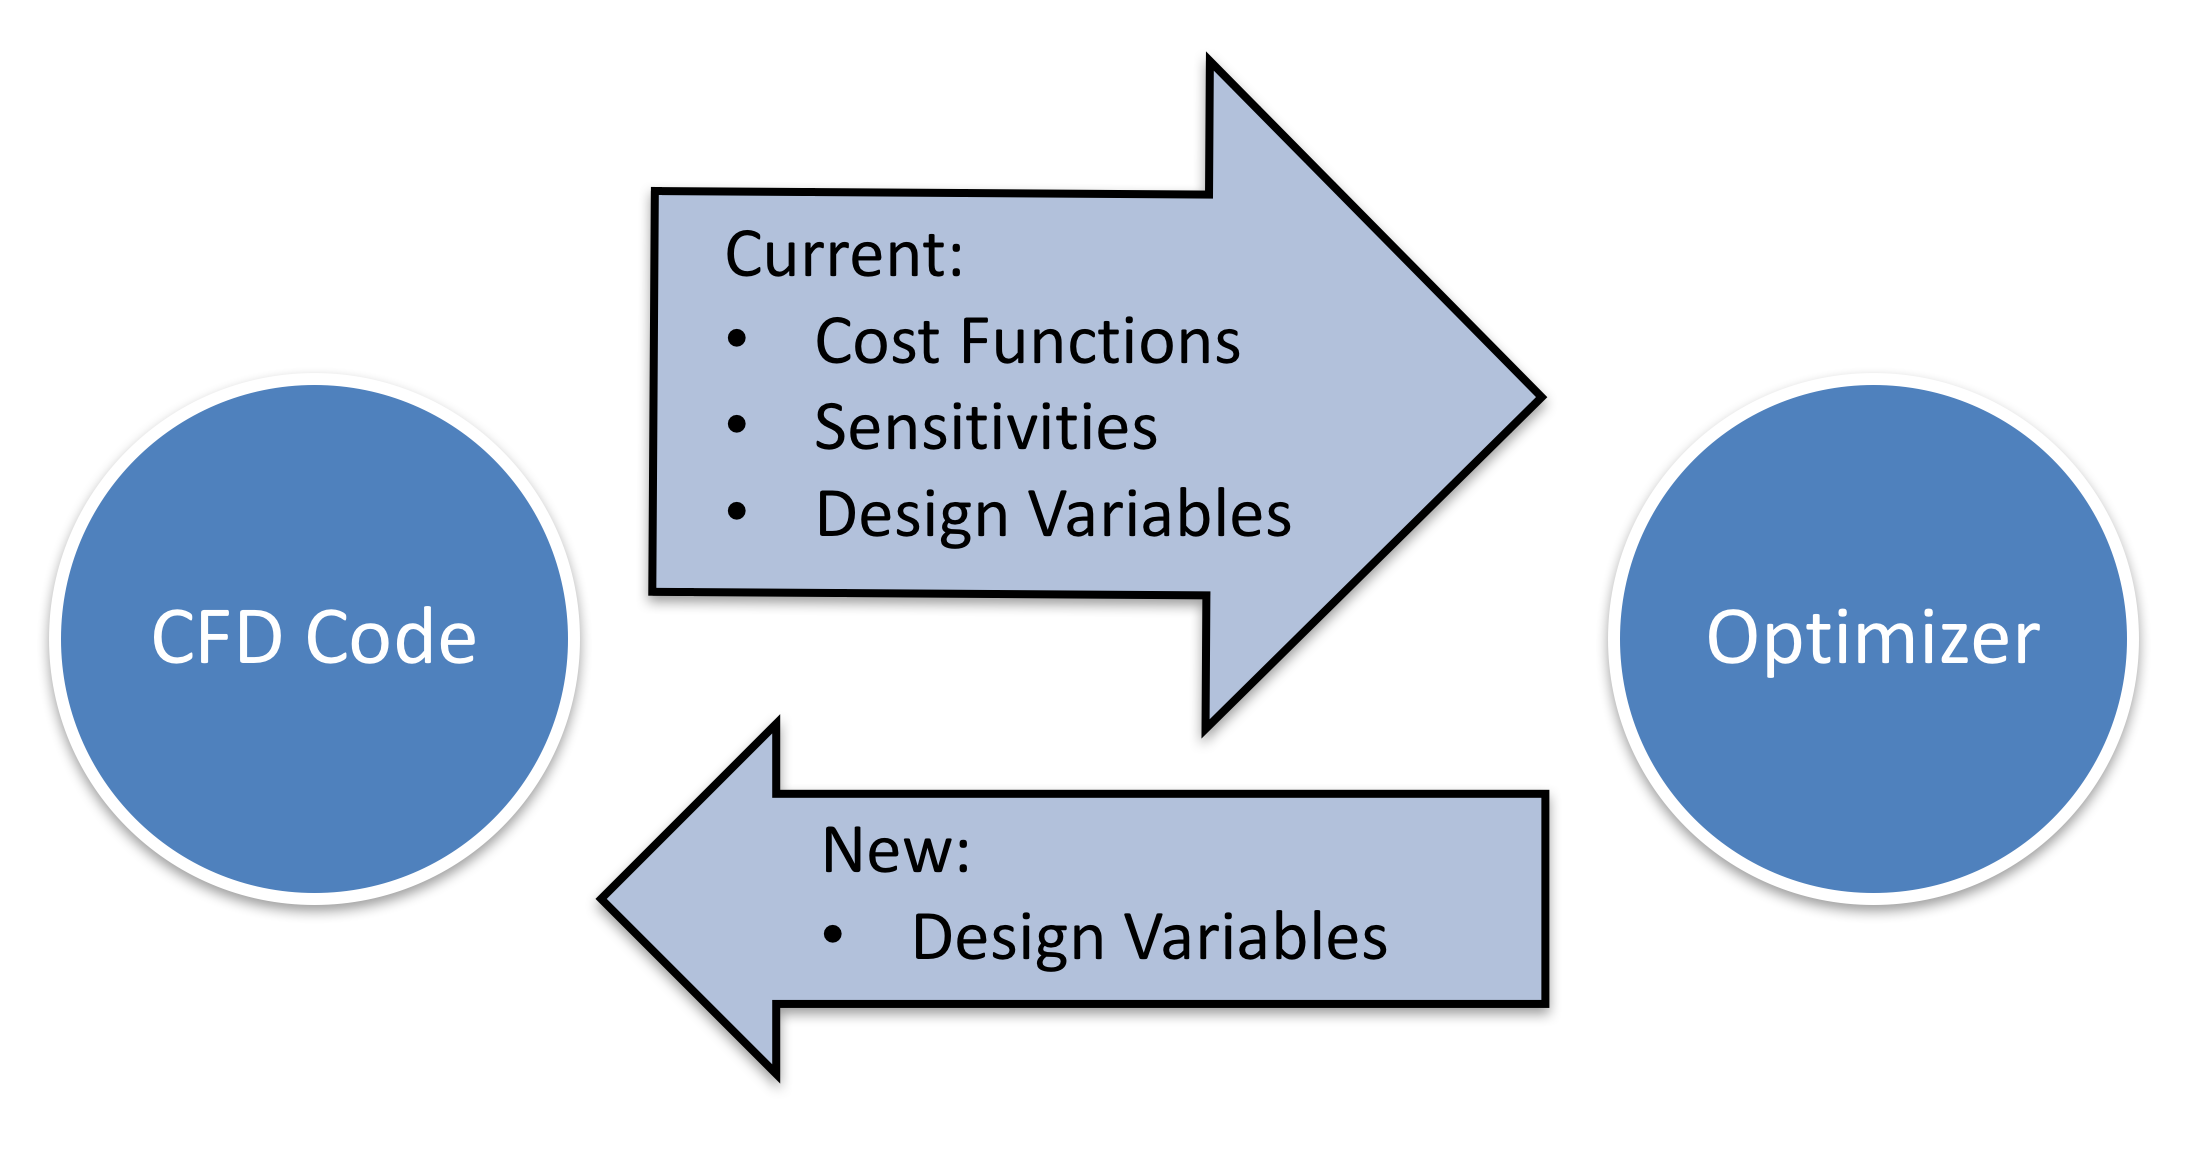
\includegraphics[width=0.6\textwidth]{figures/cfd-optimizer.png}
    \caption{CFD-Optimizer Relationship}
    \label{fig:cfd-opt}
  \end{figure}
\end{frame}
\begin{frame}
  \frametitle{Introduction - Design}
  \begin{itemize}
    \item The top-level design process is simple, but CFD sensitivity analysis 
      is expensive
    \item<2-> Need efficient way to compute cost function sensitivities for
      large number of design variables
  \end{itemize}
  \only<3>{\begin{tcolorbox}[colback=red!5!white,colframe=red!75!black, 
    title = Direct differentiation approach - Expensive]
    \begin{itemize}
      \item Navier-Stokes equations can be directly differentiated to yield
        sensitivity derivatives necessary for gradient-based optimization
      \item Finite difference requires a minimum of \textbf{one flow solution
        for each design variable sensitivity}
      \item Prohibitively expensive for large number of design variables
    \end{itemize}
  \end{tcolorbox}}
  \only<4>{\begin{tcolorbox}[colback=green!5!white,colframe=green!75!black,
    title = Adjoint approach - More efficient]
    \begin{itemize}
      \item Solve adjoint equations in addition to Navier Stokes flow equations to
        obtain sensitivity derivatives
      \item \textbf{One flow and adjoint solution needed for each cost function},
      regardless of number of design variables
      \item Considerably more efficient than direct differentiation approach for
        large number of design variables
    \end{itemize}
  \end{tcolorbox}}
\end{frame}
\begin{frame}
  \frametitle{Introduction - Design}
  \begin{itemize}
    \item Adjoint-based design optimization is widely adopted in compressible,
      perfect gas CFD solvers
    \item Reacting flow solvers have lagged in adopting adjoint-based approach,
      due to
    \begin{enumerate}
      \item Complexity of linearizing the additional equations for
        multi-species chemical kinetics
      \item Resorting to Automatic Differentiation tools incurs performance
        overhead that is implementation-specific
      \item Serious memory and computational cost concerns when simulating a
        large number of species
    \end{enumerate}
    \item Points 1 and 2 can be overcome through stubbornness (or hiring a
      graduate student\dots)
    \item Point 3 is a serious concern, if reacting flow solver are to be made
      attractive for design optimization
  \end{itemize}
\end{frame}
\begin{frame}
  \frametitle{Introduction - Improvement to State of the Art}
  \begin{itemize}
    \item Current state of the art
      \begin{itemize}
        \item Both continuous\fcite{Copeland} and
          discrete\fcite{Lockwood} adjoint formulations
          have been implemented for compressible reacting flow solvers
        \item These attempts suffer from quadratic scaling in memory and
          computational cost with number of species
        \item Recent scheme at Barcelona Supercomputing
          Center\fcite{Esfahani:2016aa} is promising, but only for
          incompressible reacting flows
      \end{itemize}
    \item Improvement to the state of the art
      \begin{itemize}
        \item New decoupled scheme for both hypersonic flow solver and adjoint
          solver that is robust for high-speed flows in chemical non-equilibrium
        \item New schemes significantly improve scaling in computational cost
          and memory with number of species
      \end{itemize}
  \end{itemize}
\end{frame}
\begin{frame}
  \frametitle{Introduction - Decoupled Approach}
  \begin{itemize}
    \item Reacting gas simulations require solving a large number of conservation
      equations
    \item Memory concerns
    \begin{itemize}
        \item Size of Jacobians scales quadratically with number species in gas mixture
        \item Solving system of equations in a tightly-coupled fashion can be
          limited by memory constraints
    \end{itemize}
    \item Cost concerns
    \begin{itemize}
      \item Cost of solving the linear system scales quadratically with number
      of species in gas mixture
    \end{itemize}
    \item Efficiently solving adjoint problem is a primary motivator
      \begin{itemize}
        \item Solving adjoint system particularly costly if linear solver is
          slow
        \item Can be necessary to store Jacobian twice $\to$ large memory
          overhead
      \end{itemize}
  \end{itemize}
\end{frame}
\begin{frame}
  \frametitle{Introduction - Decoupled Approach}
  \begin{itemize}
    \item Loosely-coupled solvers have become popular in the combustion
      community\fcite{Sankaran}
      \begin{itemize}
        \item Decouple species conservation equations from meanflow equations,
          and solve two smaller systems
         \[
           \underset{(4+ns) \times (4+ns)}
           {\begin{pmatrix}
             \boxempty & \boxempty & \dots  & \boxempty \\
             \boxempty & \boxempty & \dots  & \vdots \\
             \vdots    & \vdots    & \ddots & \vdots \\
             \boxempty & \dots     & \dots  & \boxempty
           \end{pmatrix}}
           \to
           \underset{5 \times 5}
           {\begin{pmatrix}
             \boxempty & \dots  & \boxempty \\
             \vdots    & \ddots & \vdots \\
             \boxempty & \dots  & \boxempty
           \end{pmatrix}}
           \text{and}
           \underset{ns \times ns}
           {\begin{pmatrix}
             \boxempty  & \boxbslash & \dots  & \boxbslash \\
             \boxbslash & \boxempty  & \dots  & \vdots \\
             \vdots     & \vdots     & \ddots & \vdots \\
             \boxbslash & \dots      & \dots  & \boxempty
           \end{pmatrix}}
         \]
    \end{itemize}
  \item Candler, et al.\fcite{candler} originally derived this for
    Steger-Warming scheme, this work extends to Roe FDS scheme
  \end{itemize}
\end{frame}
\begin{frame}
  \vspace{-0.2cm}
  \frametitle{Introduction - Choice of Code and Implementation}
  \begin{figure}[ht]
    \centering
    
\includegraphics[width=0.5\textwidth]{figures/fun3d_logo.png}
    \label{fig:fun3d}
  \end{figure}
  \begin{itemize}
    \item FUN3D chosen as code to facilitate all research presented, because
      \begin{itemize}
        \item Excellent infrastructure for adjoint-based design analysis and optimization
        \item Robust hypersonic flow solver
        \item NASA Langley Research Center supporting me through the Pathways
          program
      \end{itemize}
  \end{itemize}
\end{frame}

\AtBeginSection[]
{
 \begin{frame}<beamer>[shrink=20]
 \frametitle{Outline}
 \tableofcontents[currentsection]
 \end{frame}
}
\section{Flow Solver}

\subsection{Fully-Coupled Flow Solver}
\stepcounter{subsection}
\begin{frame}
  \frametitle{Fully-Coupled Point Implicit Flow Solver}
  \begin{itemize}
    \item All work presented is for inviscid flows in chemical non-equilibrium,
      using a one-temperature model, but is extendable to viscous flows.
    \item Finite-volume with backward-Euler time integration
    \begin{equation*}
    	\label{inv_flux_fv}
    	\frac{\partial \mU}{\partial t}
    	 + \frac{1}{\vol}\sum\limits_{f}(\vF \cdot \Norm)^f = \mw
    \end{equation*}
    \begin{equation*}
    	\begin{matrix}
    	\mU=\begin{pmatrix}
       		\rho_1\\
    		\vdots \\
    		\rho_{N_s} \\
    		\rho \vu \\
    		\rho E \\
    	\end{pmatrix},      &
     	\vF \cdot \Norm = \begin{pmatrix}
    		\rho_1  \overline{U} \\
    		\vdots \\
    		\rho_{N_s} \overline{U} \\
    		\rho \vu \overline{U} + p \norm \\
    		(\rho E + p) \overline{U} \\
    	\end{pmatrix} N,    &
     	\mw = \begin{pmatrix}
        \dot\rho_1\\
    		\vdots \\
    		\dot\rho_{N_s} \\
        0 \\
        0
      \end{pmatrix}

  	\end{matrix}
  \end{equation*}

  \end{itemize}
\end{frame}
\begin{frame}
  \frametitle{Fully-Coupled Point Implicit Flow Solver}
  \begin{itemize}
  \item<1-> Using the Roe FDS scheme to compute the inviscid flux at the face,
    $\vF^f$, and linearizing the system results in an implicit system 
    \begin{equation*}
      \left( \frac{\vol}{\Delta t} \mi + \druduapprox \right)\Delta \mU = \ru{}
    \end{equation*}
  \item<2-> With global system composed of block matrices
%------------------------------------------------------------------------------%
  \begin{sequation}[0.8]
  \underbrace{
    \left[ 
      \frac{\vol}{\Delta t} \mi + 
      \begin{pmatrix}
        \rdiff{\rho_1}{\rho_1}     & \dots  & \rdiff{\rho_1}{\rho_{N_s}}     & \rdiff{\rho_1}{\rho \vu}     & \rdiff{\rho_1}{\rho E}      \\
        \vdots                     & \ddots & \vdots                         & \vdots                       & \vdots                      \\
        \rdiff{\rho_{N_s}}{\rho_1} & \dots  & \rdiff{\rho_{N_s}}{\rho_{N_s}} & \rdiff{\rho_{N_s}}{\rho \vu} &  \rdiff{\rho_{N_s}}{\rho E} \\
        \rdiff{\rho \vu}{c_1}      & \dots  & \rdiff{\rho \vu}{c_{N_s}}      & \rdiff{\rho \vu}{\rho \vu}   &  \rdiff{\rho \vu}{\rho E}   \\
        \rdiff{\rho E}{c_1}        & \dots  & \rdiff{\rho E}{c_{N_s}}        & \rdiff{\rho E}{\rho \vu}     &  \rdiff{\rho E}{\rho E}
      \end{pmatrix}
    \right]
  }_\text{$(N_s + 4) \times (N_s + 4)$}
  \underbrace{
    \begin{pmatrix}
      \Delta \mU_{\rho_1}     \\[4pt]
      \vdots                  \\[4pt]
      \Delta \mU_{\rho_{N_s}} \\[4pt]
      \Delta \mU_{\rho \vu}   \\[4pt]
      \Delta \mU_{\rho E}
    \end{pmatrix}
  }_\text{$(N_s + 4) \times 1$}
  =
  \underbrace{
    \begin{pmatrix}
      \res{\rho_1}     \\[4pt]
      \vdots           \\[4pt]
      \res{\rho_{N_s}} \\[4pt]
      \res{\rho \vu}   \\[4pt]
      \res{\rho E}
    \end{pmatrix}
  }_\text{$(N_s + 4) \times 1$}
  \end{sequation}
%------------------------------------------------------------------------------%
  \end{itemize}
\end{frame}
\begin{frame}
  \frametitle{Fully-Coupled Point Implicit Flow Solver}
  \begin{itemize}
    \item Constructing the Jacobian in a fully-coupled fashion results in large,
      dense block matrices
    \item Cost of multi-color Gauss-Seidel sweeps dominated by matrix-vector
      products 
      \[
        \text{Cost} \to O((N_s + 4)^2)
      \]
    \item Leads to onerous quadratic scaling with respect to number of species
  \end{itemize}
\end{frame}

\subsection{Decoupled Flow Solver}
\stepcounter{subsection}

\begin{frame}
  \frametitle{Decoupled Point Implicit Flow Solver}
  \begin{itemize}
    \item The main idea is to separate the meanflow and species composition
      equations, adding a new equation for the total mixture density
    \item Leads to two sets of conserved variables
      \begin{equation*}
      	\begin{matrix}
      		\Up =\begin{pmatrix}
      			\rho \\
      			\rho u \\
      			\rho v \\
      			\rho w \\
      			\rho E
      		\end{pmatrix} &
      		\Vhat = \begin{pmatrix}
      			c_1 \\
      			\vdots \\
      			c_{N_s}
      		\end{pmatrix} \\ \\
          \text{Meanflow} & \text{Species Composition}
      	\end{matrix} 
      \end{equation*}
  \end{itemize}
\end{frame}

\begin{frame}
  \frametitle{Decoupled Point Implicit Flow Solver}
  \begin{itemize}
    \item The Roe FDS scheme species mass fluxes can be rewritten as
      \begin{align*}
  	    \Fhat_{\rho_s}
          &= 
        \tilde{c}_s 
        \only<1>{
          \begin{cboxf}[white]
            \vF'_{\rho}
          \end{cboxf}
        }
        \only<2>{
          \begin{cboxf}[green]
            \vF'_{\rho}
          \end{cboxf}
        }
        + (c_s^L-\tilde{c}_s)\rho^L\lambda^+ 
        + (c_s^R-\tilde{c}_s)\rho^R\lambda^- \\
        \pd{\Fhat_{\rho_s}}{c_s^L} 
          &= 
        \roe 
        \only<1>{
          \begin{cboxf}[white]
            \vF'_{\rho}
          \end{cboxf}
        }
        \only<2>{
          \begin{cboxf}[green]
            \vF'_{\rho}
          \end{cboxf}
        }
        + (1-\roe)\rho^L\lambda^+ - \roe \rho^R\lambda^- \\
        \pd{\Fhat_{\rho_s}}{c_s^R} 
        	&=
        (1-\roe)
        \only<1>{
          \begin{cboxf}[white]
            \vF'_{\rho}
          \end{cboxf}
        }
        \only<2>{
          \begin{cboxf}[green]
            \vF'_{\rho}
          \end{cboxf}
        }
        +(\roe-1)\rho^L\lambda^+ + \roe \rho^R\lambda^-
      \end{align*}
    \item Jacobian Approximations
      \begin{align*}
	\text{Step 1:}\quad &
	\frac{\partial \vF}{\partial \mU'}\bigg|_{\mathbf{\hat{V}}} =
	\underset{c_s = \text{Constant}}{5 \times 5\,\text{Roe FDS Jacobian}} \\
	\text{Step 2:}\quad & 
	\frac{\partial \vF}{\partial \hat{\mv}}\bigg|_{\mathbf{\hat{U'}}} = 
        \begin{pmatrix} 
          \frac{\partial F_{\rho_1}}{\partial c_1} & & 0
          \\ & \ddots &  \\ 0 & & \frac{\partial F_{\rho_{ns}}}{\partial c_{ns}}
        \end{pmatrix} 
      \end{align*}
  \end{itemize}
\end{frame}
\begin{frame}
  \frametitle{Decoupled Point Implicit Flow Solver}
  \vspace{-0.5cm}
  \small
%------------------------------------------------------------------------------%
\begin{gather*}
    \text{\bf{Mixture Equations}}: \\
    \left[ 
    \frac{\vol}{\Delta t}\mi + \drup
    \right] \Delta \Up
  =
  \res{\Up} \\
  \left[ 
    \frac{\vol}{\Delta t}\mi + 
    \begin{pmatrix}
      \rdiff{\rho}{\rho} & \rdiff{\rho}{\rho \vu} & \rdiff{\rho}{\rho E} \\
      \rdiff{\rho \vu}{\rho} & \rdiff{\rho \vu}{\rho \vu} & \rdiff{\rho \vu}{\rho E} \\
      \rdiff{\rho E}{\rho} & \rdiff{\rho E}{\rho \vu} & \rdiff{\rho E}{\rho E}
    \end{pmatrix}
  \right]
  \begin{pmatrix}
    \Delta \rho \\
    \Delta \rho \vu \\
    \Delta \rho E
  \end{pmatrix}
  =
  \begin{pmatrix}
    \resrho \\
    \res{\rho \vu} \\
    \res{\rho E}
  \end{pmatrix} \\[12pt]
    \text{\bf{Species Continuity Equations}}: \\
    \left[ 
    \frac{\vol}{\Delta t}\mi + \drvhat
    \right] \Delta \Vhat
    =
    \res{\Vhat} \\
  \left[
    \frac{\rho \vol}{\Delta t}\mi + 
    \begin{pmatrix}
      \rdiff{\rho_1}{c_1} & \cdots & \rdiff{\rho_{1}}{c_{ns}} \\
      \vdots & \ddots & \vdots \\
      \rdiff{\rho_{ns}}{c_1} & \cdots & \rdiff{\rho_{ns}}{c_{ns}}
    \end{pmatrix}
  \right]
  \begin{pmatrix}
    \Delta c_1 \\
    \vdots \\
    \Delta c_{ns}
  \end{pmatrix}
  =
  \begin{pmatrix}
    \res{\rho_1} - c_1 \resrho \\
    \vdots \\
    \res{\rho_{N_s}} - c_{N_s} \resrho
  \end{pmatrix}
\end{gather*}
%------------------------------------------------------------------------------%
\end{frame}

\subsection{Cost and Memory Savings of the Decoupled Flow Solver}

\begin{frame}
  \frametitle{Cost and Memory Savings of the Decoupled Flow Solver}
\begin{itemize}
  \item Most significant savings comes from the source term linearization being purely node-based
    \begin{itemize}
      \item Convective contributions to block Jacobians are diagonal
      \item Source term Jacobian is dense block Jacobian
      \item In the global system (w/chemistry), all off-diagonal block Jacobians
        are diagonal
    \end{itemize}
  \end{itemize}
  \begin{sequation}[0.8]
    \begin{pmatrix} 
      \Box & & & & \\ 
      & \ddots & & & \\ 
      & & \Box \\ 
      & & & \ddots & \\ 
      & & & & \Box
    \end{pmatrix}
    \begin{pmatrix} 
      \delta \mathbf{\hat{V}}_1 \\ 
      \vdots \\ 
      \delta \mathbf{\hat{V}}_i \\ 
      \vdots \\
      \delta \mathbf{\hat{V}}_{nodes}
    \end{pmatrix}^{n+1}
    = 
    \begin{pmatrix} 
      \hat{b}_1 \\ 
      \vdots \\ 
      \hat{b}_i \\ 
      \vdots \\
      \hat{b}_{nodes} 
    \end{pmatrix}
    - 
    \begin{pmatrix}
      (\sum_{j=1}^{N_{nb}}{[\diagdown] \delta\mathbf{\hat{V}}_{j}})_1 \\ 
      \vdots \\
      (\sum_{j=1}^{N_{nb}}{[\diagdown] \delta\mathbf{\hat{V}}_{j}})_i \\ 
      \vdots \\
      (\sum_{j=1}^{N_{nb}}{[\diagdown] \delta\mathbf{\hat{V}}_{j}})_{nodes}
    \end{pmatrix}^{n,n+1}
  \end{sequation}
  \begin{itemize}
    \item Diagonal matrix-vector product operations similar to vector inner
      product operations: $O(N_s^2) \to O(N_s)$
  \end{itemize}
\end{frame}
\begin{frame}
  \frametitle{Cost and Memory Savings of the Decoupled Flow Solver}
  \begin{itemize}
    \item Comparing size of Jacobian systems, using Compressed Row Storage
  \end{itemize}
  \begin{align*}
    \ma_d &= \text{Decoupled system Jacobians} \\
    \ma &= \text{Fully-coupled system Jacobians}
  \end{align*}
  \[
  \begin{split} Relative\ Memory\ Cost &=
    \frac{size(\ma_d)}{size(\ma)} \\ &= \lim_{N_s\to\infty}
    \frac{(N_s^2+5^2)(N_{nodes})+(N_s+5^2)(N_{nbrs})}{(N_s+4)^2(N_{nodes}+N_{nbrs})} \\
    &= \frac{N_{nodes}}{N_{nodes} + N_{nbrs}}
  \end{split}
  \]
\end{frame}


\section{Adjoint Solver}
\stepcounter{subsection}
\subsection{Derivation of Discrete Adjoint Formulation}
\begin{frame}
  \frametitle{Derivation of Discrete Adjoint Formulation}
  \begin{itemize}
    \item The derivation of the adjoint approach to compute design sensitivities
      begins with forming the Lagrangian and differentiating with respect to the
      design variables
      \begin{gather*}
        L(\md,\mq,\adjlam{})=f(\md,\mq)
        +\adjlam{}^T\mr(\md,\mq) \\
        \uncover<2->{
       	\pd{L}{\md} =
        \pd{f}{\md} +
        \only<2>{
        \begin{cboxf}[white]
          \left[ \pd{\mq}{\md} \right]^T
          \left\{\pd{f}{\mq} + \left[ \pd{\mr}{\mq} \right]^T \adjlam{} \right\}
        \end{cboxf}
        }
        \only<3>{
        \begin{cboxf}[green]
          \left[ \pd{\mq}{\md} \right]^T
          \left\{\pd{f}{\mq} + \left[\pd{\mr}{\mq}\right]^T \adjlam{} \right\}
        \end{cboxf}
        }
       	+ \left[\pd{\mr}{\md}\right]^T \adjlam{}} \\
        \begin{aligned} 
          \md &= \text{design variables}\quad & f &= \text{cost function} \\
          \mq &= \text{flow variables}\quad & \mr &= \text{flow residual} \\ 
        \end{aligned} \\
        \adjlam{} = \text{costate variables} 
      \end{gather*}
  \end{itemize}
\end{frame}
\begin{frame}
    \frametitle{Derivation of Discrete Adjoint Formulation}
    \begin{itemize}
      \item Need to eliminate flow variable dependence on design variables,
	$\pd{\mq}{\md}$
      \item Adjoint equation
        \[ \bigg[\pd{\mr}{\mq}\bigg]^T\adjlam{} = -\pd{f}{\mq} \]
      \item Solve for $\adjlam{}$ and compute sensitivity derivatives
      	\[
          \pd{L}{\md} = \pd{f}{\md} + \left[ \rdiff{}{\md} \right]^T \adjlam{}
      	\]
    \end{itemize}
\end{frame}

\subsection{Fully Coupled Adjoint Solver}

\begin{frame}
  \frametitle{Fully Coupled Adjoint Solver}
  \begin{itemize}
    \item Adjoint problem is a linear system
      \begin{equation*}
        \begin{pmatrix}
          \rtdiff{\rho_i}{\rho_j} & 
          \rtdiff{\rho \vu}{\rho_j} & 
          \rtdiff{\rho E}{\rho_j} \\
          \\
          \rtdiff{\rho_i}{\rho \vu} & 
          \rtdiff{\rho \vu}{\rho \vu} & 
          \rtdiff{\rho E}{\rho \vu} \\
          \\
          \rtdiff{\rho_i}{\rho E} &
          \rtdiff{\rho \vu}{\rho E} &
          \rtdiff{\rho E}{\rho E}
        \end{pmatrix}
        \begin{pmatrix}
          \adjlam{\rho_i} \\ \\
          \adjlam{\rho \vu} \\ \\
          \adjlam{\rho E}
        \end{pmatrix}
        = -
        \begin{pmatrix}
          \pd{f}{\rho_i} \\ \\
          \pd{f}{\rho \vu} \\ \\
          \pd{f}{\rho E}
        \end{pmatrix}
      \end{equation*}
    \item Can be solved with Krylov method (i.e. GMRES), but time marching
      similar to flow solver shown to be more robust
      \begin{equation*}
        \left( \frac{\vol}{\Delta t} \mi + \druduapprox \right)^{\mathsmaller T}
        \Delta \adjlam{}
        = - \left( \rtdiff{\mU}{\mU} \adjlam{\mU}^{n} + \pd{f}{\mU} \right)
      \end{equation*}
    \item Straightforward to formulate, but cost and memory requirements
      scale quadratically with number of species
      
  \end{itemize}
\end{frame}

\subsection{Decoupled Adjoint Method}

\begin{frame}
  \frametitle{Decoupled Adjoint Scheme}
  \begin{itemize}
    \item The decoupled flow solver has an analog in the adjoint
    \item First, recognize that the decoupled flow solver can be rewritten as a
      fully coupled system, with a change of variables and change of equations
  \end{itemize}
  %------------------------------------------------------------------------------%
  \begin{sequation}[0.85]
    \underbrace{
      \mU = \begin{pmatrix}
        \rho_1 \\
        \vdots \\
        \rho_{ns} \\
        \rho \vu \\
        \rho E
      \end{pmatrix}
      \rightarrow
      \mv = \begin{pmatrix}
        c_1 \\
        \vdots \\
        c_{ns} \\
        \rho \\
        \rho \vu \\
        \rho E
      \end{pmatrix}
    }_\text{Change of Variables}
      ,\quad
    \underbrace{
      \ru{} =
      \begin{pmatrix}
        \res{\rho_1} \\
        \vdots \\
        \res{\rho_{N_s}} \\
        \res{\rho \vu} \\
        \res{\rho E}
      \end{pmatrix}
      \rightarrow
      \rv{} =
      \begin{pmatrix}
        \res{\rho_1} - c_1 \resrho \\
        \vdots \\
        \res{\rho_{N_s}} - c_{N_s} \resrho \\
        \resrho \\
        \res{\rho \vu} \\
        \res{\rho E}
      \end{pmatrix}
    }_\text{Change of Equations}
    \label{fc-to-dc-res}
  \end{sequation}
  %------------------------------------------------------------------------------%
  \begin{equation*}
    c_s = \frac{\rho_s}{\rho}, \quad \rho = \lsum{i=1}{N_s}{\left( \rho_i \right)}
  \end{equation*}
\end{frame}
\begin{frame}
  \frametitle{Decoupled Adjoint Scheme}
  \begin{itemize}
    \item This change of variables/equations results in non-square transformation
      matricies
  \end{itemize}
  \vspace{0.5cm}
%------------------------------------------------------------------------------%
\begin{sequation}[0.8]
  \pd{\mU}{\mv} = 
  \begin{pmatrix}
    \rho   & \dots  & 0      & c_1     & 0      & 0      \\
    \vdots & \ddots & \vdots & \vdots  & \vdots & \vdots \\
    0      & \dots  &\rho    & c_{ns}  & 0      & 0      \\
    0      & \dots  &0       & 0       & 1      & 0      \\
    0      & \dots  &0       & 0       & 0      & 1
  \end{pmatrix}, \ 
  \pd{\rv{}}{\ru{}} =
  \begin{pmatrix}
    1 - c_1  & -c_1     & \dots  & -c_1      & 0      & 0      \\
    -c_2     & 1-c_2    & \dots  & -c_2      & 0      & 0      \\
    \vdots   & \vdots   & \ddots & \vdots    & \vdots & \vdots \\
    -c_{N_s} & -c_{N_s} & \dots  & 1-c_{N_s} & 0      & 0      \\
    1        & 1        & \dots  & 1         & 0      & 0      \\
    0        & 0        & \dots  & 0         & 1      & 0      \\
    0        & 0        & \dots  & 0         & 0      & 1      \\
  \end{pmatrix}
\end{sequation}
%------------------------------------------------------------------------------%
\end{frame}
\begin{frame}
  \frametitle{Decoupled Adjoint Scheme}
  \begin{itemize}
    \item<1-> Using the transformation matricies, $\pd{\mU}{\mv}$ and
      $\pd{\ru{}}{\rv{}}$, it possible to treat the decoupled approach as a
      series of matrix operations
      \begin{equation*}
        \pd{\rv{}}{\mv} = \pd{\rv{}}{\ru{}} \pd{\ru{}}{\mU} \pd{\mU}{\mv}
      \end{equation*}
    \item<2-> These matrix operations can be thought of as left and right
      preconditioning
      \begin{equation*}
        \pd{\rv{}}{\mv} = 
        \underbrace{ \left(\pd{\rv{}}{\ru{}}\right) }_{\text{Left Preconditioner}}
        \left(\pd{\ru{}}{\mU}\right)
        \underbrace{ \left(\pd{\mU}{\mv}\right) }_{\text{Right Preconditioner}}
      \end{equation*}
    \item<3-> This transformation avoids having to explicitly form the Jacobian
      $\pd{\rv{}}{\mv}$, which is more complicated than $\pd{\ru{}}{\mU}$
  \end{itemize}
\end{frame}
\begin{frame}
  \frametitle{Decoupled Adjoint Scheme}
  \begin{itemize}
    \item Rewrite the adjoint system from 
      $\ru{}\left( \mU \right) \only<2->{\rightarrow \rv{}\left( \mv \right)}$
      \begin{gather*}
        \left( \pd{\ru{}}{\mU} \right)^T \adjlam{\mU} = -\pd{f}{\mU} \\
        \only<2->{
          \left( \pd{\mU}{\mv} \right)^T 
          \left( \pd{\ru{}}{\mU} \right)^T 
          \left( \pd{\rv{}}{\ru{}} \right)^T 
          \adjlam{\mv} = -\left( \pd{\mU}{\mv} \right)^T
          \left(\pd{f}{\mU}\right)
        }
      \end{gather*}
    \item<3-> Effectively another Left/Right Preconditioning
  \end{itemize}
  \vspace{0.2cm}
  \only<3->{
  \begin{sequation}[0.9]
    \underbrace{
      \left( \pd{\mU}{\mv} \right)^T 
    }_\text{Left Preconditioning}
    \left( \pd{\ru{}}{\mU} \right)^T 
    \underbrace{
      \left( \pd{\rv{}}{\ru{}} \right)^T \adjlam{\mv}
    }_\text{Right Preconditioning}
    = -
    \underbrace{
      \left( \pd{\mU}{\mv} \right)^T
    }_\text{Left Preconditioning}
    \left(\pd{f}{\mU}\right)
  \end{sequation}
  \begin{sequation}[0.9]
    \left( \pd{\rv{}}{\ru{}} \right)^T \adjlam{\mv} = \adjlam{\mU}
  \end{sequation}
  }
\end{frame}
\begin{frame}
  \frametitle{Decoupled Adjoint Solver}
  \begin{itemize}
    \item Time march adjoint solution with approximate Jacobians
      \begin{equation*}
        \left( \frac{\vol}{\Delta t} \mi + \drvdvapprox^T \right) \adjlam{\mv}
        =
        - \left( \pd{\mU}{\mv} \right)^T
        \underbrace{
          \left( \pd{\ru{}}{\mU} \adjlam{\mU} + \pd{f}{\mU} \right)
        }_\text{Fully Coupled Residual}
      \end{equation*}
    \item Split $\drvdv$ in same fashion as flow solver
  \end{itemize}
  \only<2>{\begin{sequation}[0.6]
    \begin{pmatrix}
      \rpdiff{\rho_1}{c_1} & \dots & \rpdiff{\rho_1}{c_{N_s}} &
      \rpdiff{\rho_1}{\rho} &
      \rpdiff{\rho_1}{\rho \vu} & 
      \rpdiff{\rho_1}{\rho E}  \\
      \\
      \vdots & \ddots & \vdots & \vdots & \vdots & \vdots \\
      \\
      \rpdiff{\rho_{N_s}}{c_1}  & \dots  & \rpdiff{\rho_{N_s}}{c_{N_s}} & 
      \rpdiff{\rho_{N_s}}{\rho} & 
      \rpdiff{\rho_{N_s}}{\rho \vu} &
      \rpdiff{\rho_{N_s}}{\rho E} \\
      \\
      \rdiff{\rho}{c_1} & \dots & \rdiff{\rho}{c_{N_s}} &
      \rdiff{\rho}{\rho} & 
      \rdiff{\rho}{\rho \vu} & 
      \rdiff{\rho}{\rho E} \\
      \\
      \rdiff{\rho \vu}{c_1} & \dots  & \rdiff{\rho \vu}{c_{N_s}} &
      \rdiff{\rho \vu}{\rho} &
      \rdiff{\rho \vu}{\rho \vu} &
      \rdiff{\rho \vu}{\rho E} \\
      \\
      \rdiff{\rho E}{c_1} & \dots & \rdiff{\rho E}{c_{N_s}} &
      \rdiff{\rho E}{\rho} &
      \rdiff{\rho E}{\rho \vu} &
      \rdiff{\rho E}{\rho E}
    \end{pmatrix}
  \end{sequation}}
  \only<3>{\begin{sequation}[0.6]
    \begin{parray}[6]
      \tikzmark{left}{$\rpdiff{\rho_1}{c_1}$} & \dots & \rpdiff{\rho_1}{c_{N_s}} &
      \rpdiff{\rho_1}{\rho} &
      \rpdiff{\rho_1}{\rho \vu} & 
      \rpdiff{\rho_1}{\rho E}  \\
      \\
      \vdots & \ddots & \vdots & \vdots & \vdots & \vdots \\
      \\
      \rpdiff{\rho_{N_s}}{c_1}  & \dots  &
      \tikzmark{right}{$\rpdiff{\rho_{N_s}}{c_{N_s}}$} & 
      \rpdiff{\rho_{N_s}}{\rho} & 
      \rpdiff{\rho_{N_s}}{\rho \vu} &
      \rpdiff{\rho_{N_s}}{\rho E} \\
      \Rhighlight[dc-jac]
      \\
      \rdiff{\rho}{c_1} & \dots & \rdiff{\rho}{c_{N_s}} &
      \tikzmark{left}{$\rdiff{\rho}{\rho}$} & 
      \rdiff{\rho}{\rho \vu} & 
      \rdiff{\rho}{\rho E} \\
      \\
      \rdiff{\rho \vu}{c_1} & \dots  & \rdiff{\rho \vu}{c_{N_s}} &
      \rdiff{\rho \vu}{\rho} &
      \rdiff{\rho \vu}{\rho \vu} &
      \rdiff{\rho \vu}{\rho E} \\
      \\
      \rdiff{\rho E}{c_1} & \dots & \rdiff{\rho E}{c_{N_s}} &
      \rdiff{\rho E}{\rho} &
      \rdiff{\rho E}{\rho \vu} &
      \tikzmark{right}{$\rdiff{\rho E}{\rho E}$}
      \Bhighlight[fc-jac]
    \end{parray}
  \end{sequation}}
  \only<4>{\begin{sequation}[0.6]
    \begin{parray}[6]
      \tikzmark{left}{$\rpdiff{\rho_1}{c_1}$} & \dots & \rpdiff{\rho_1}{c_{N_s}} &
      \rpdiff{\rho_1}{\rho} &
      \rpdiff{\rho_1}{\rho \vu} & 
      \rpdiff{\rho_1}{\rho E}  \\
      \\
      \vdots & \ddots & \vdots & \vdots & \vdots & \vdots \\
      \\
      \rpdiff{\rho_{N_s}}{c_1}  & \dots  &
      \tikzmark{right}{$\rpdiff{\rho_{N_s}}{c_{N_s}}$} & 
      \rpdiff{\rho_{N_s}}{\rho} & 
      \rpdiff{\rho_{N_s}}{\rho \vu} &
      \rpdiff{\rho_{N_s}}{\rho E} \\
      \Rhighlight[dc-jac]
      \\
      \rdiff{\rho}{c_1} & \dots & \rdiff{\rho}{c_{N_s}} &
      \tikzmark{left}{$\rdiff{\rho}{\rho}$} & 
      \rdiff{\rho}{\rho \vu} & 
      \rdiff{\rho}{\rho E} \\
      \\
      \rdiff{\rho \vu}{c_1} & \dots  & \rdiff{\rho \vu}{c_{N_s}} &
      \rdiff{\rho \vu}{\rho} &
      \rdiff{\rho \vu}{\rho \vu} &
      \rdiff{\rho \vu}{\rho E} \\
      \\
      \rdiff{\rho E}{c_1} & \dots & \rdiff{\rho E}{c_{N_s}} &
      \rdiff{\rho E}{\rho} &
      \rdiff{\rho E}{\rho \vu} &
      \tikzmark{right}{$\rdiff{\rho E}{\rho E}$}
      \Bhighlight[fc-jac]
    \end{parray}
    \rightarrow
    \overbrace{
      \begin{parray}[3]
        \tikzmark{left}{$\rdiff{\rho_1}{c_1}$} & \dots & \rdiff{\rho_1}{c_{N_s}} \\
        \vdots & \ddots & \vdots \\
        \rdiff{\rho_{N_s}}{c_1}  & \dots &
        \tikzmark{right}{$\rdiff{\rho_{N_s}}{c_{N_s}}$}
      \end{parray}
    }^\text{\huge $\drvhat$}
    \Nohighlight[dc-jac2]
    , \quad
    \overbrace{
    \begin{parray}[3]
      \tikzmark{left}{$\rdiff{\rho}{\rho}$} & \rdiff{\rho}{\rho \vu} &
      \rdiff{\rho}{\rho E} \\ \\
      \rdiff{\rho \vu}{\rho} & \rdiff{\rho \vu}{\rho \vu} & \rdiff{\rho
      \vu}{\rho E} \\ \\
      \rdiff{\rho E}{\rho} & \rdiff{\rho E}{\rho \vu} &
      \tikzmark{right}{$\rdiff{\rho E}{\rho E}$}
    \end{parray}
    }^\text{\huge $\drup$}
    \Nohighlight[fc-jac2]
    \tikz[overlay,remember picture] {
      \draw[->,thick,red,dashed] (dc-jac) -- (dc-jac2) 
      node [pos=0.45,sloped,above] {Species Equations};
    }
    \tikz[overlay,remember picture] {
      \draw[->,thick,blue,dashed] (fc-jac) .. controls (-3,-2.5) .. (fc-jac2) 
      node [pos=0.2,sloped,above] {Mixture Equations};
    }
  \end{sequation}}
\end{frame}

\begin{frame}
  \frametitle{Decoupled Adjoint Solver}
  \begin{itemize}
    \item Separate into two systems and solve as block Jacobi scheme
  \end{itemize}
%------------------------------------------------------------------------------%
\begin{gather*}
  \text{\bf{Species Continuity Equations}}: \\
  \begin{cboxn}[red]
    \left(
    \frac{\rho \vol}{\Delta t} \mi + \pd{\mathbf{\tilde{R}_{\Vhat}}}{\Vhat}
    \right)^{\mathsmaller T} \Delta \adjlam{\Vhat}
    =
    - \left( \pd{\mU}{\Vhat} \right)^{\mathsmaller T}
    \left(\pd{\ru{}}{\mU}^{\mathsmaller T}\adjlam{\mU}^n + \pd{f}{\mU} \right)
  \end{cboxn} \\
  \text{\bf{Mixture Equations}}: \\
  \begin{cboxn}[blue]
    \left(
    \frac{\vol}{\Delta t} \mi + \pd{\mathbf{\tilde{R}_{\Up}}}{\Up}
    \right)^{\mathsmaller T} \Delta \adjlam{\Up}
    =
    - \left( \pd{\mU}{\Up} \right)^{\mathsmaller T}
    \left(\pd{\ru{}}{\mU}^{\mathsmaller T}\adjlam{\mU}^n + \pd{f}{\mU} \right)
  \end{cboxn}
\end{gather*}
\end{frame}

\section{Annular Jet}
\subsection{Geometry and Test Conditions}
\begin{frame}
  \frametitle{Geometry and Test Conditions}
  \begin{columns}
    \begin{column}{0.4\textwidth}
    %------------------------------------------------------------------------------%
      \vspace{-0.5cm}
    \begin{figure}
      \centering
      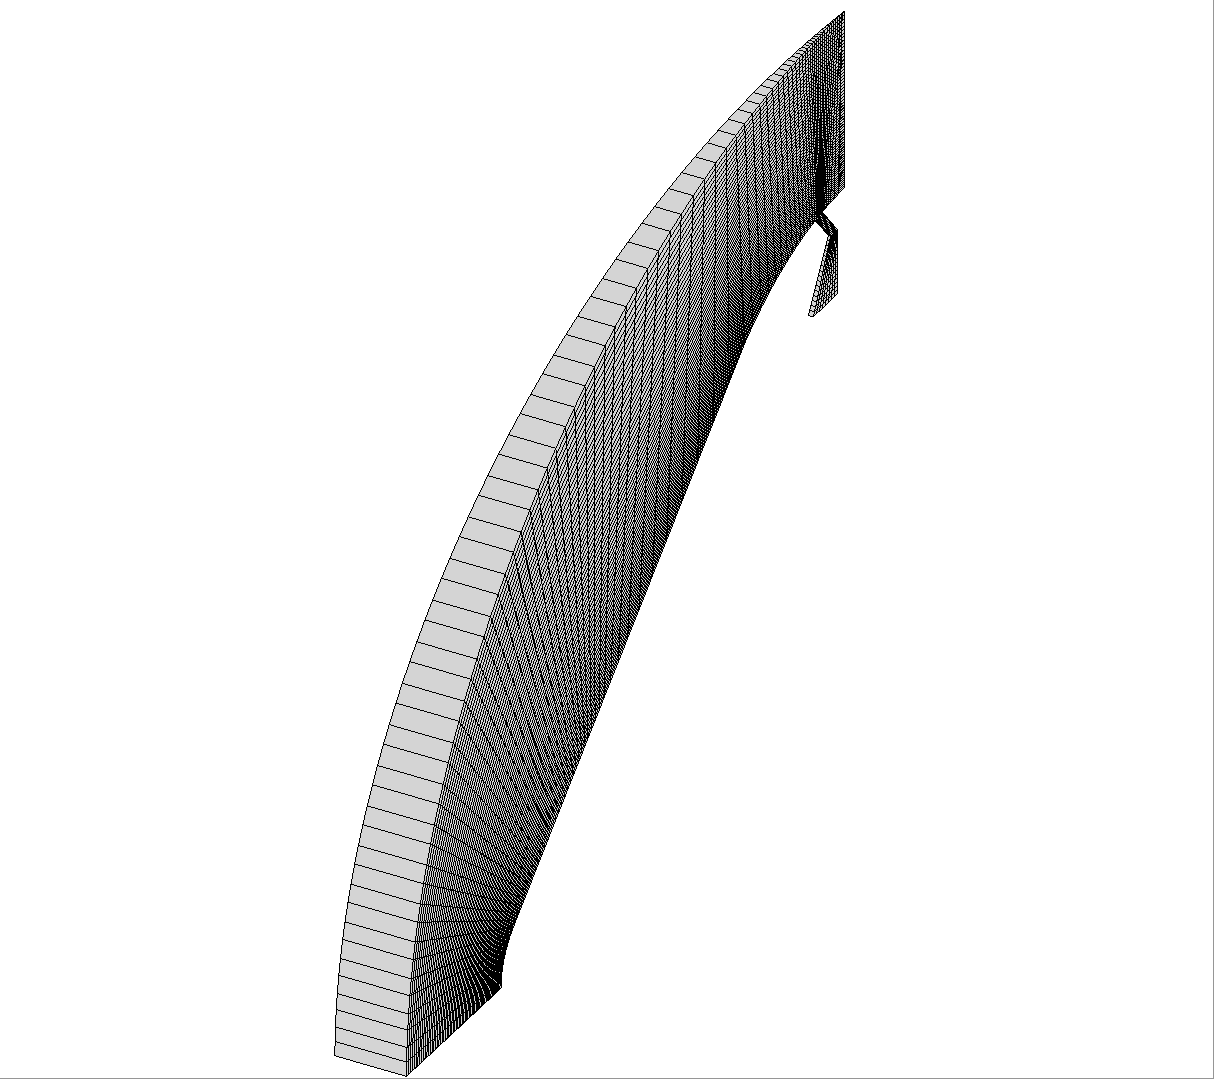
\includegraphics[width=0.7\textwidth]{figures/iso-coarse.png}
    \end{figure}
    \vspace{-0.75cm}
    \begin{figure}
      \centering
        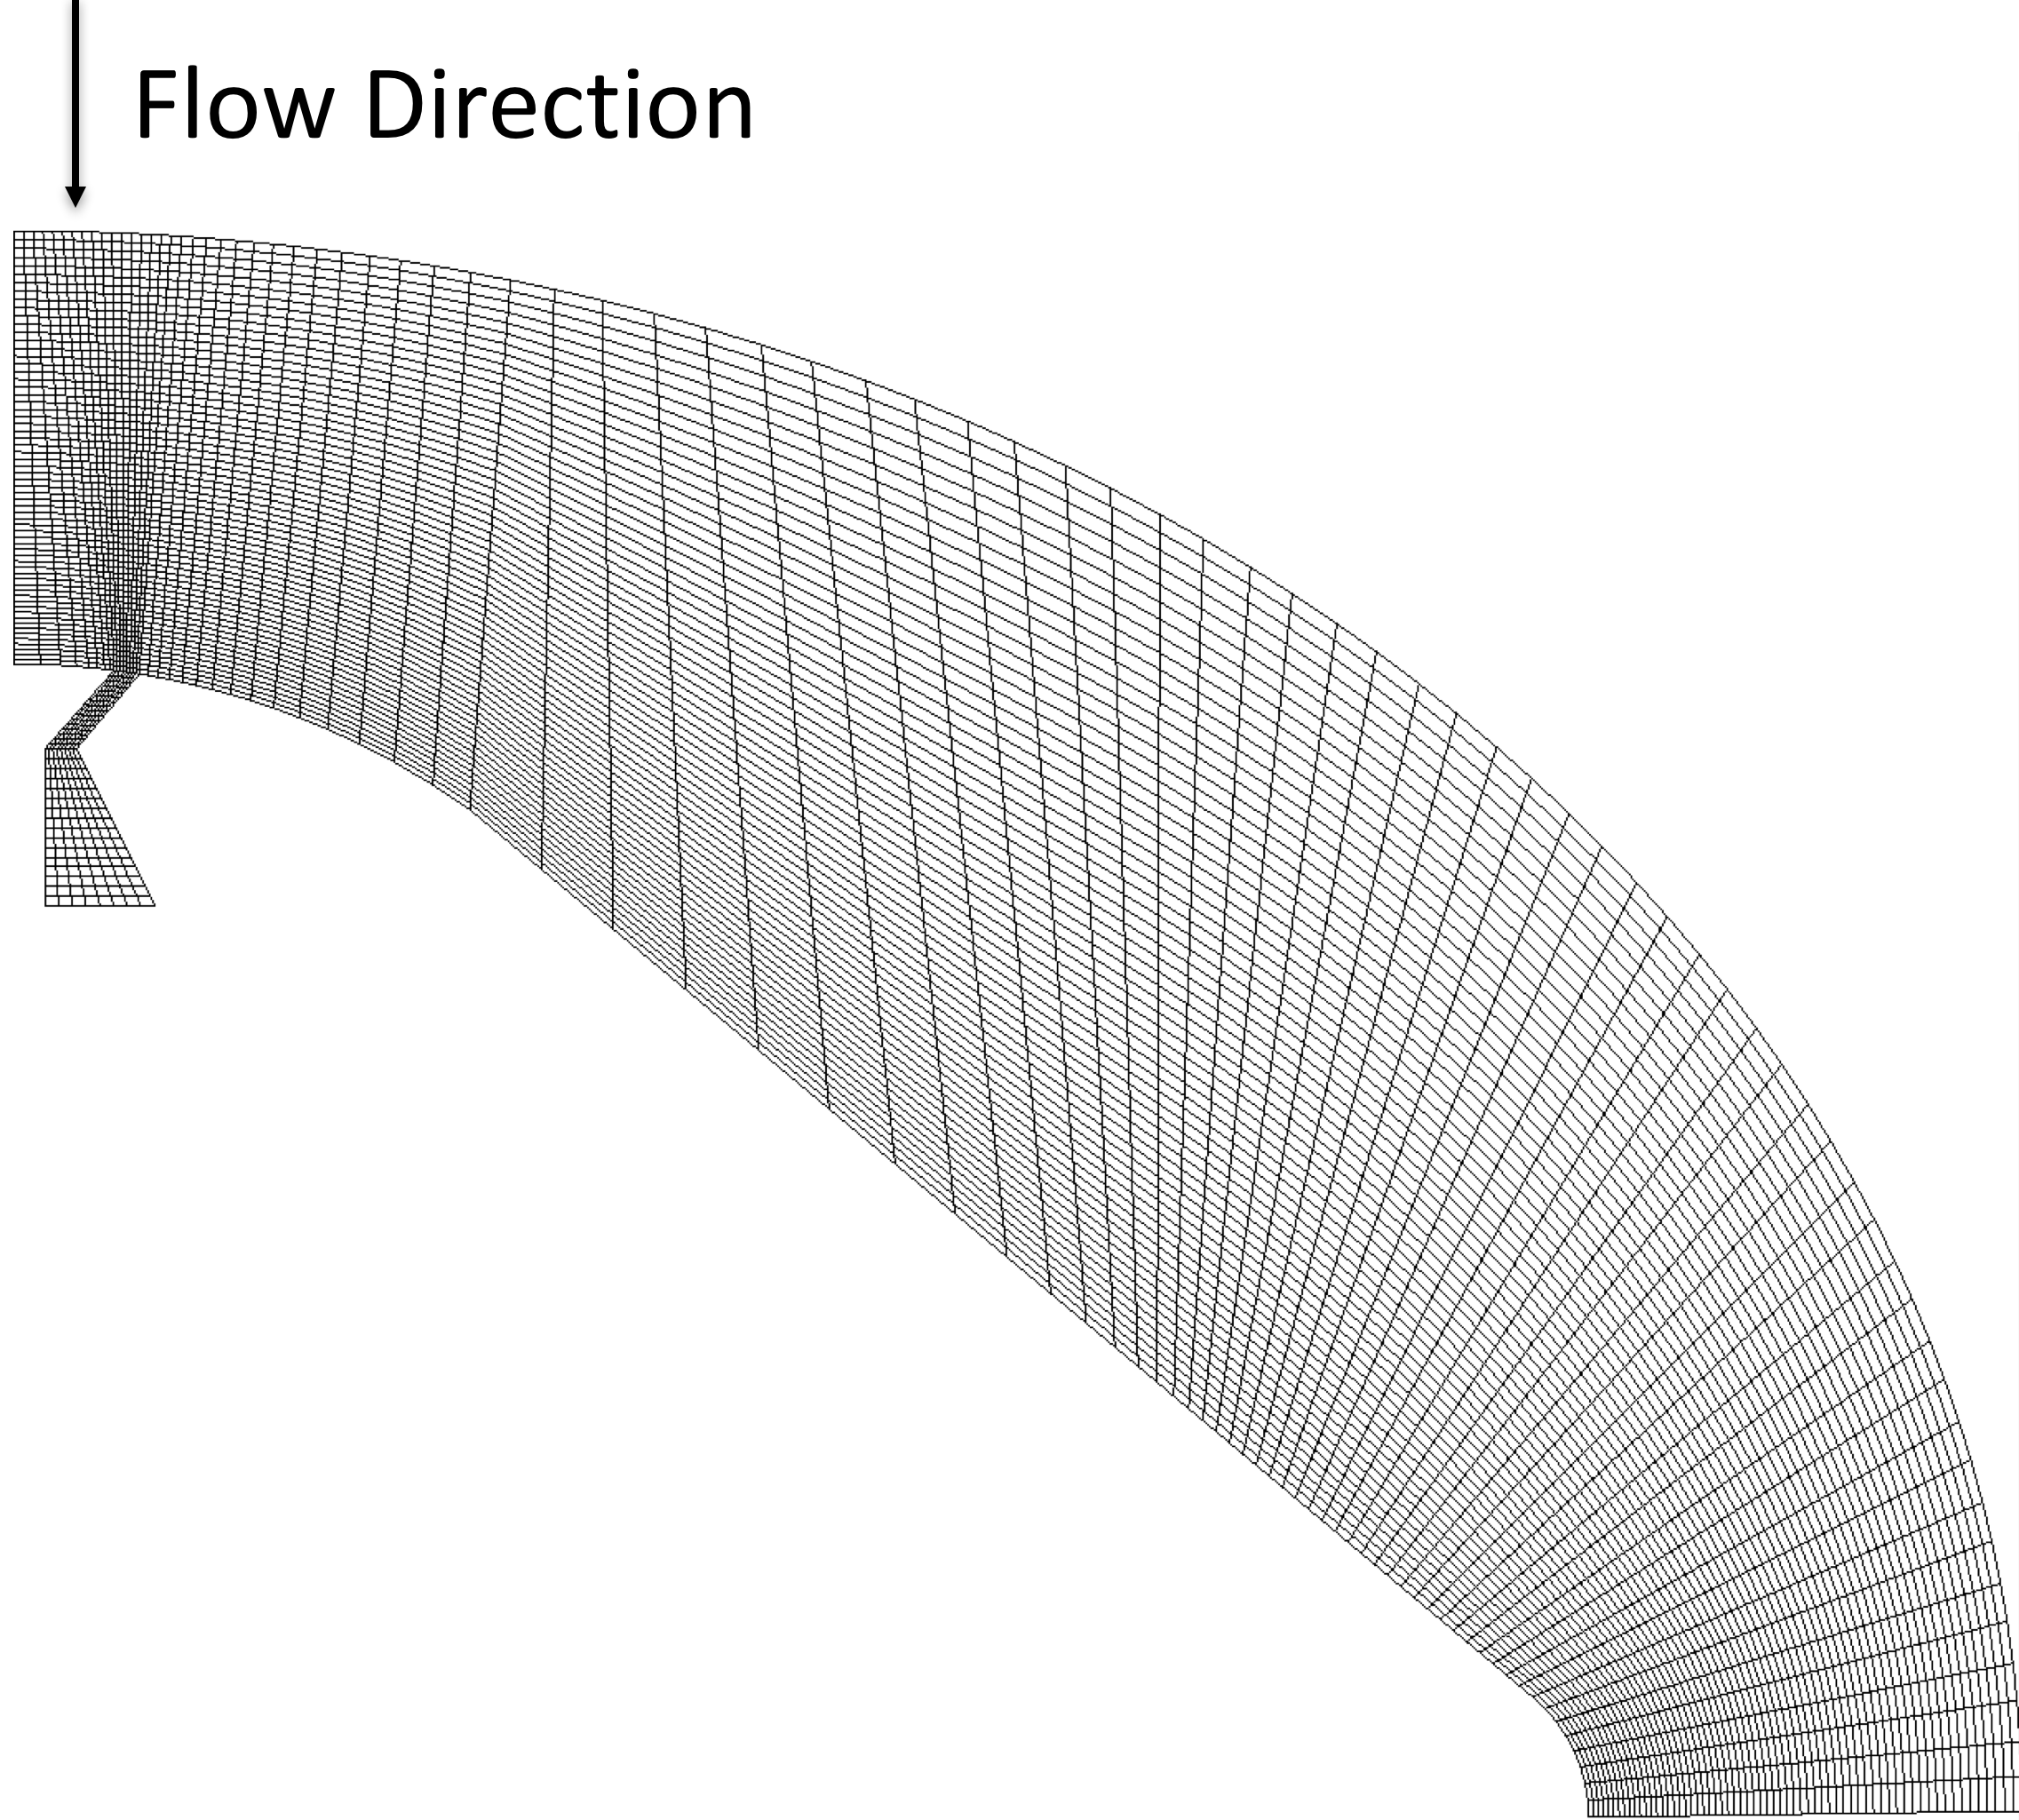
\includegraphics[width=\textwidth]{figures/side-coarse-flowdir.png}
      \caption{Annular jet geometry.}
    \end{figure}
    %------------------------------------------------------------------------------%
    \end{column}
    \begin{column}{0.65\textwidth}
    %------------------------------------------------------------------------------%
    \begin{table}[!h]
      \tiny
      \centering
      \begin{tabular}{c|c|c}
        Flow Condition & Description & Value \\
        \hline
        $V_{\infty}$    & freestream velocity, $m/s$        & 5686.24 \\
        $\rho_{\infty}$ & freestream density, $kg/m^3$      & 0.001 \\
        $T_{\infty}$    & freestream temperature, $K$       & 200.0 \\
        $M_{\infty}$    & freestream Mach number (derived)  & 20.0
      \end{tabular}
      \caption{Flow conditions.}
      \label{tab:flow-conditions}
    \end{table}
    %------------------------------------------------------------------------------%
    \vspace{-0.5cm}
    \small
     \begin{itemize}
       \item Requirements of demonstration problem:
         \begin{itemize}
           \item Steady flow
           \item Hypersonic flow condition with challenging physics
           \item Chemical non-equilibrium
         \end{itemize}
       \item Extending hypersonic retro-propulsion work by Gnoffo et al. from
         perfect gas simulation to hydrogen-air mixture meets these requirements
    \end{itemize}
    \end{column}
  \end{columns}
\end{frame}
\subsection{Flow Features and Cone Angle Effects}
\begin{frame}
  \frametitle{Flow Features and Cone Angle Effects}
\only<1>{
  \begin{itemize}
    \item Flow separates downstream of nozzle exit, creating a buffer gas zone
      of relatively low temperature.
  \end{itemize}
  \vspace{-0.4cm}
%------------------------------------------------------------------------------%
\begin{figure}[h!]
  \centering
  \subfloat[$70^o$ Cone angle]{
    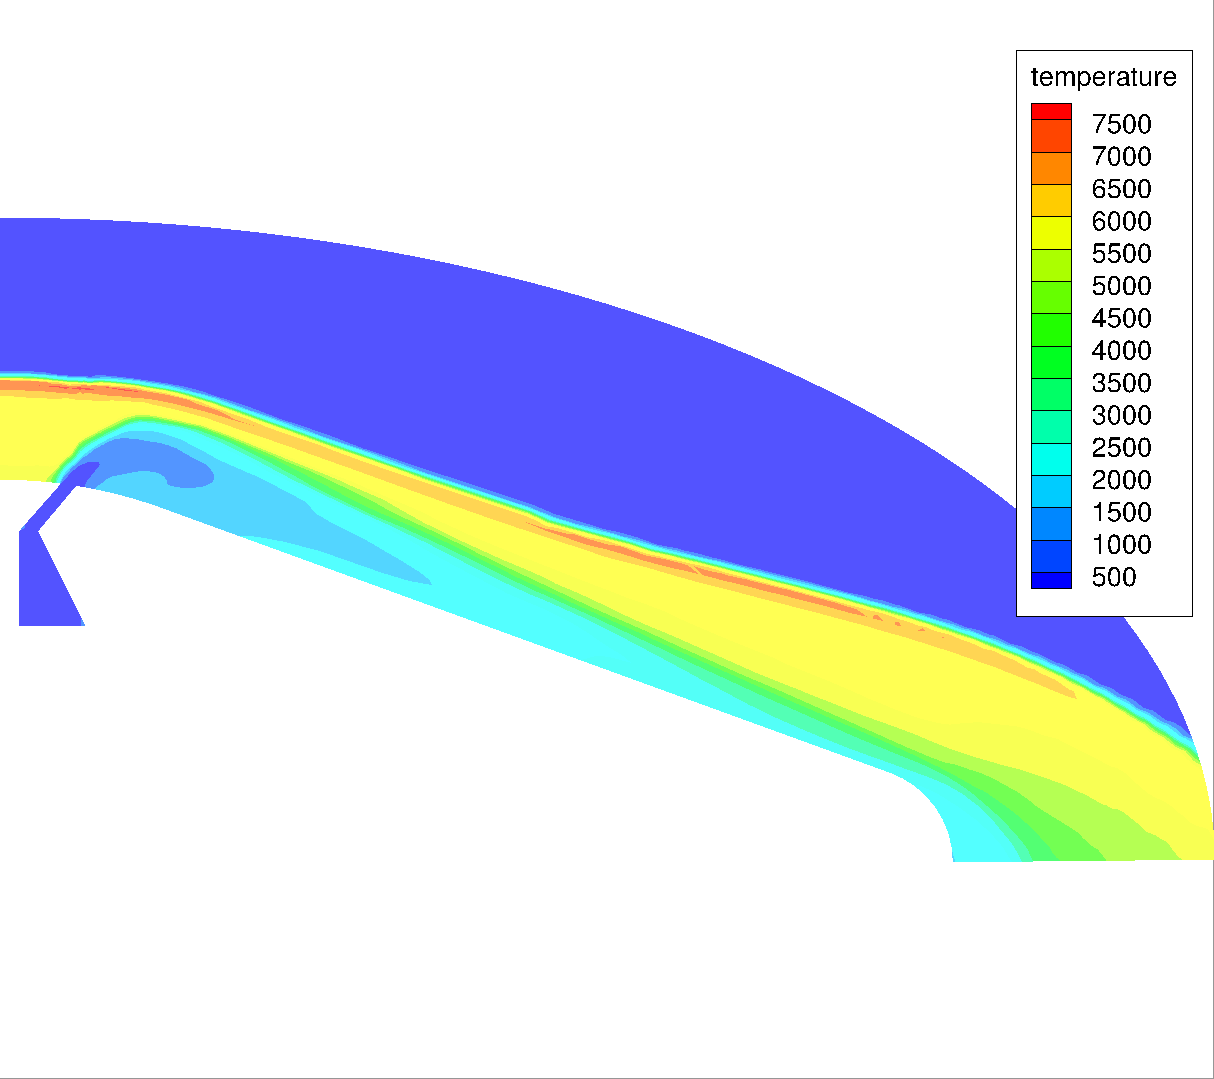
\includegraphics[width=0.45\textwidth]{figures/srp/70deg-temperature.png}}
  \subfloat[$50^o$ Cone angle]{
    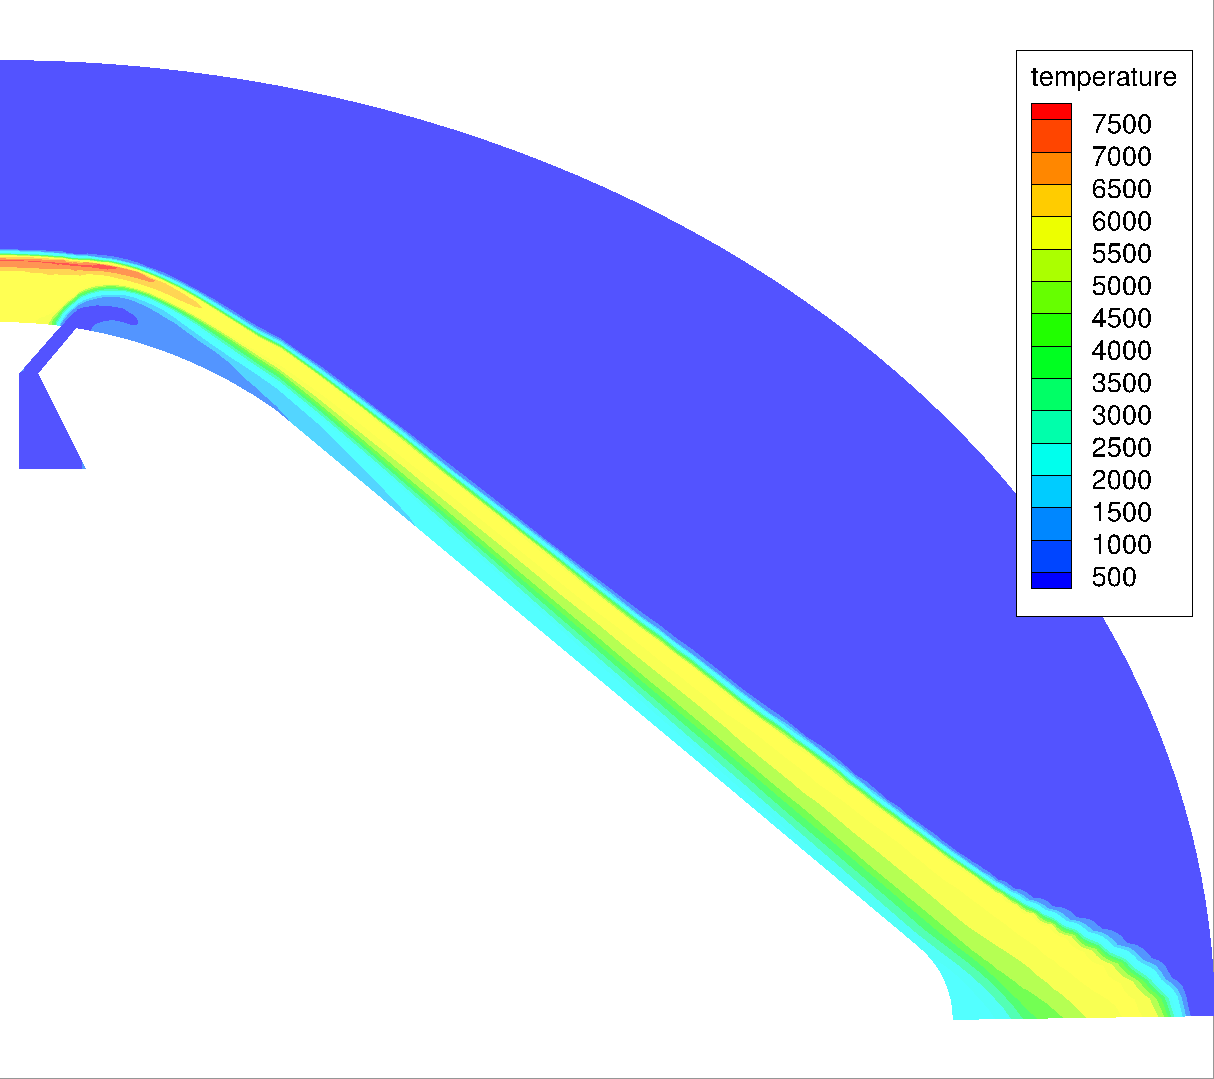
\includegraphics[width=0.45\textwidth]{figures/srp/50deg-temperature.png}}
  \caption{Annular jet temperature contours, blowing pure $H_2$.}
\end{figure}
%------------------------------------------------------------------------------%
}
\only<2>{
  \begin{itemize}
    \item Strong dependence between cone angle and size of recirculation zone
  \end{itemize}
  \vspace{-0.4cm}
%------------------------------------------------------------------------------%
\begin{figure}[h!]
  \centering
  \subfloat[$70^o$ Cone angle]{
    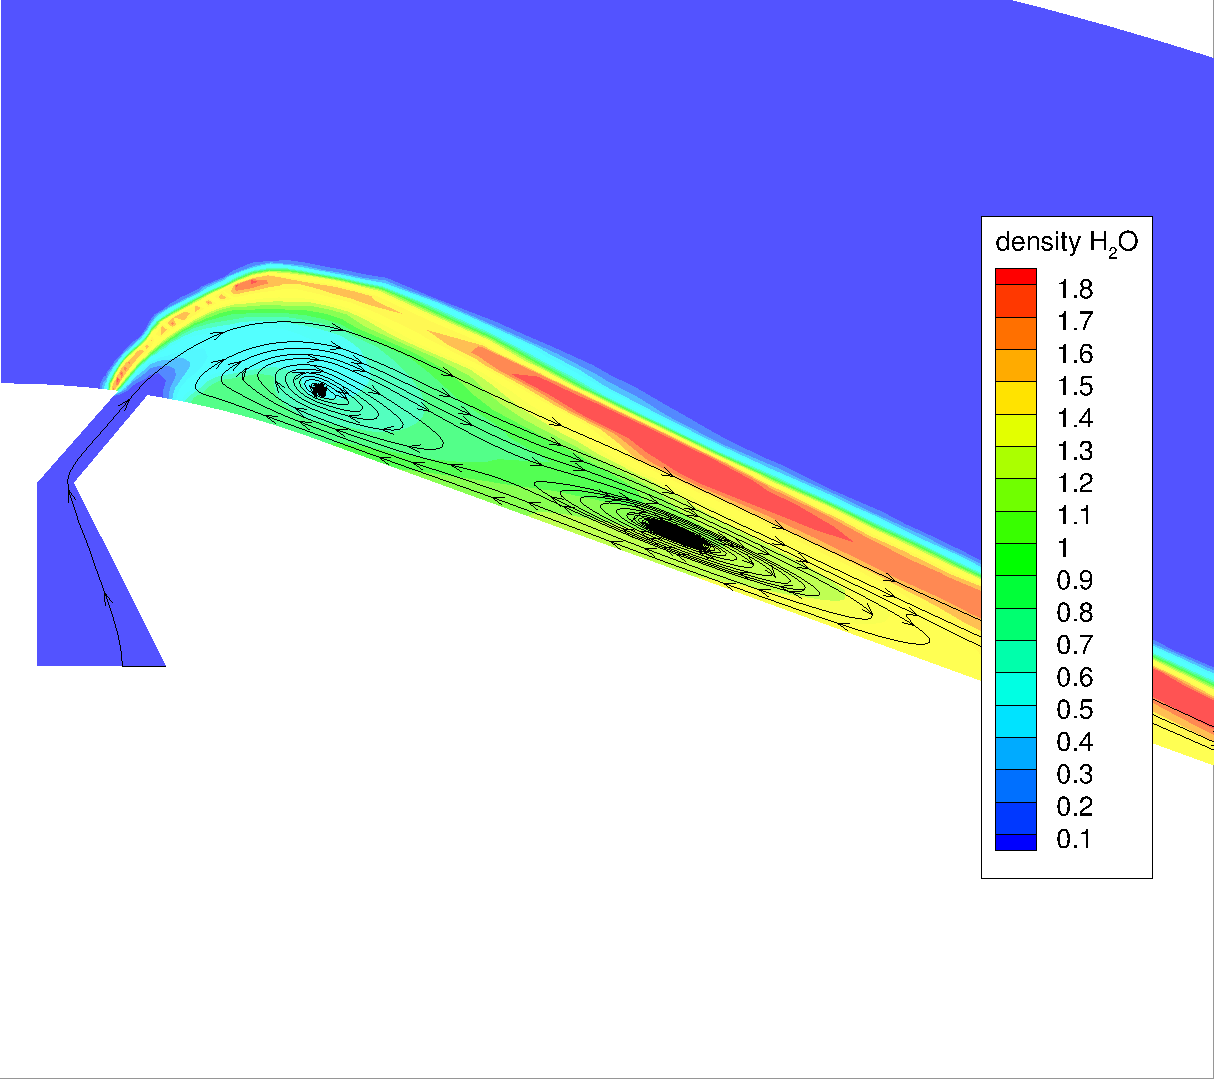
\includegraphics[width=0.45\textwidth]{figures/srp/70deg-water.png}}
  \subfloat[$50^o$ Cone angle]{
    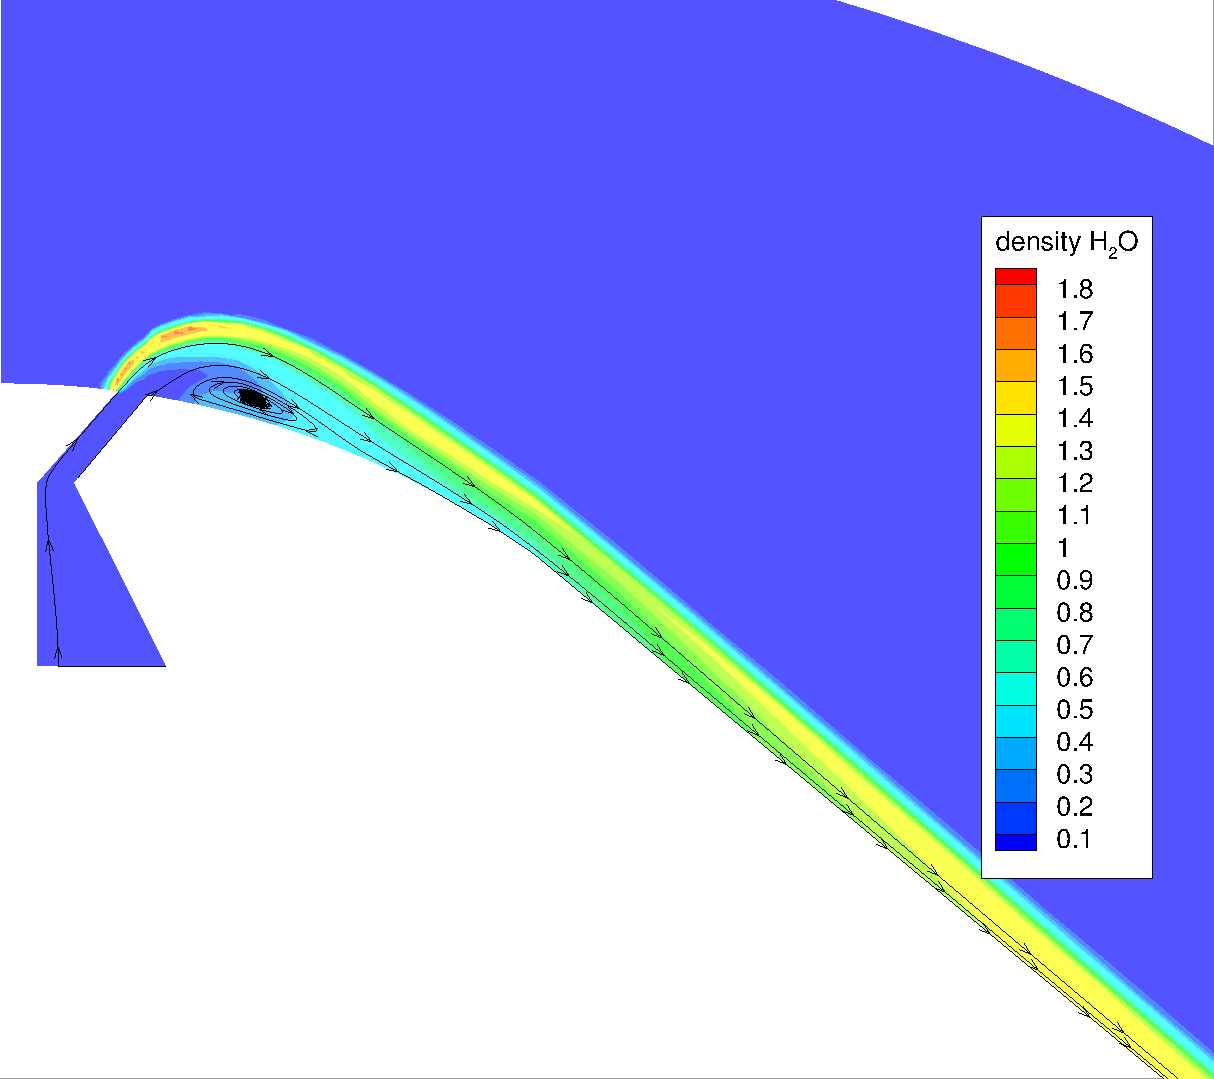
\includegraphics[width=0.45\textwidth]{figures/srp/50deg-water.png}}
  \caption{Annular jet $H_2 O$ density contours, blowing pure $H_2$.}
\end{figure}
%------------------------------------------------------------------------------%
}
\only<3>{
  \begin{itemize}
    \item $70^o$ Cone angle leads to sonic-corner body with low-amplitude
      oscillations in the separation bubble
  \end{itemize}
  \vspace{-0.4cm}
%------------------------------------------------------------------------------%
\begin{figure}[h!]
  \centering
  \subfloat[$70^o$ Cone angle]{
    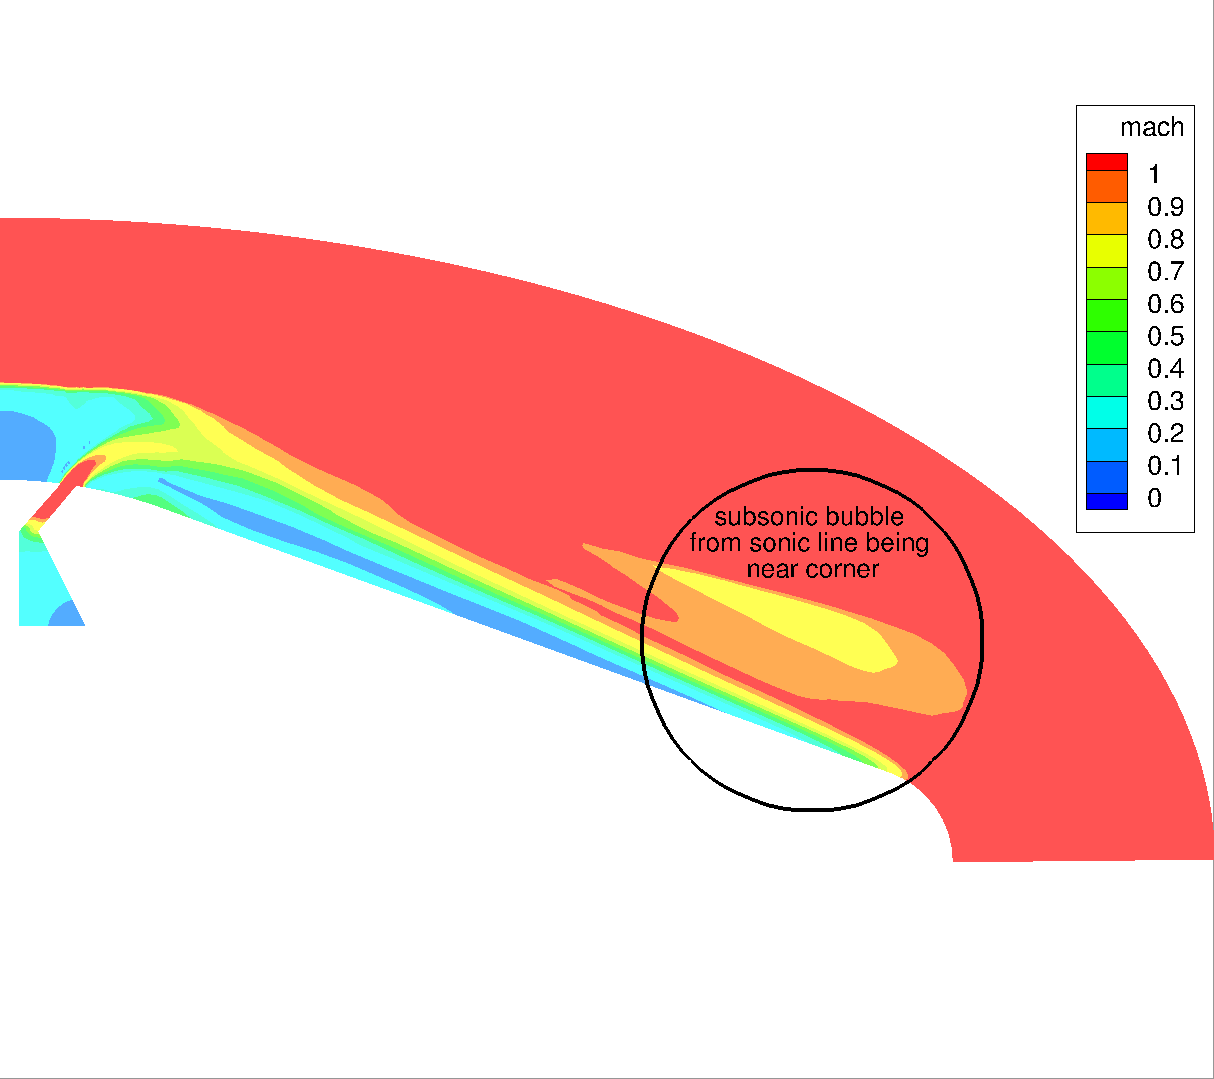
\includegraphics[width=0.45\textwidth]{figures/sonic-bubble/sonic_bubble.png}}
  \subfloat[$50^o$ Cone angle]{
    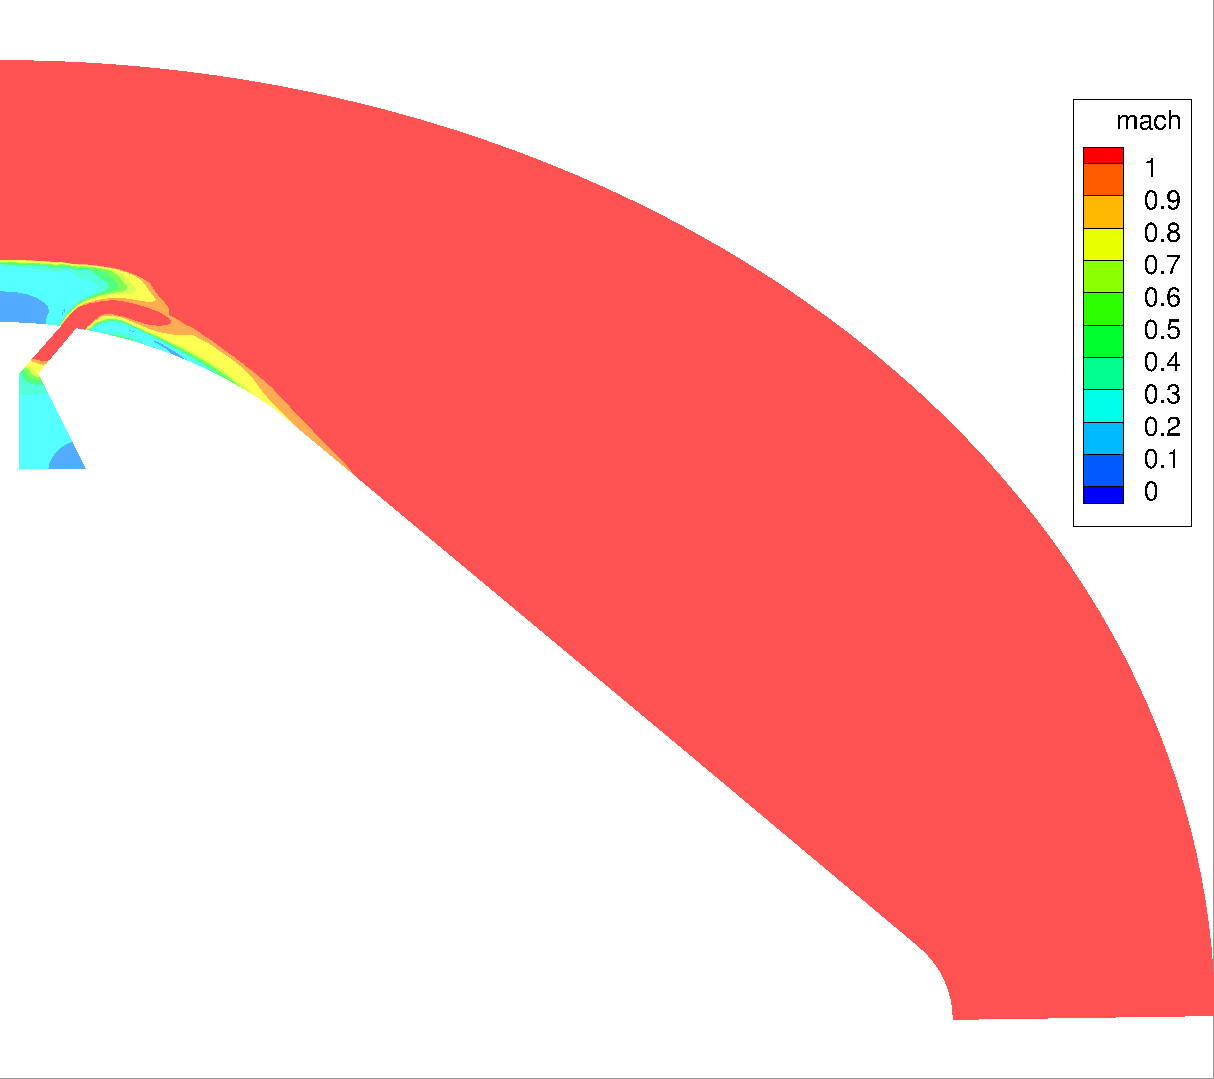
\includegraphics[width=0.45\textwidth]{figures/sonic-bubble/no_bubble.png}}
  \caption{Annular jet sonic line comparison, blowing pure $H_2$.}
\end{figure}
%------------------------------------------------------------------------------%
}
\end{frame}
\subsection{Solution Sensitivity to Mesh Density}
\begin{frame}
  \frametitle{Solution Sensitivity to Mesh Density}
  %------------------------------------------------------------------------------%
  \begin{figure}[h]
    \centering
    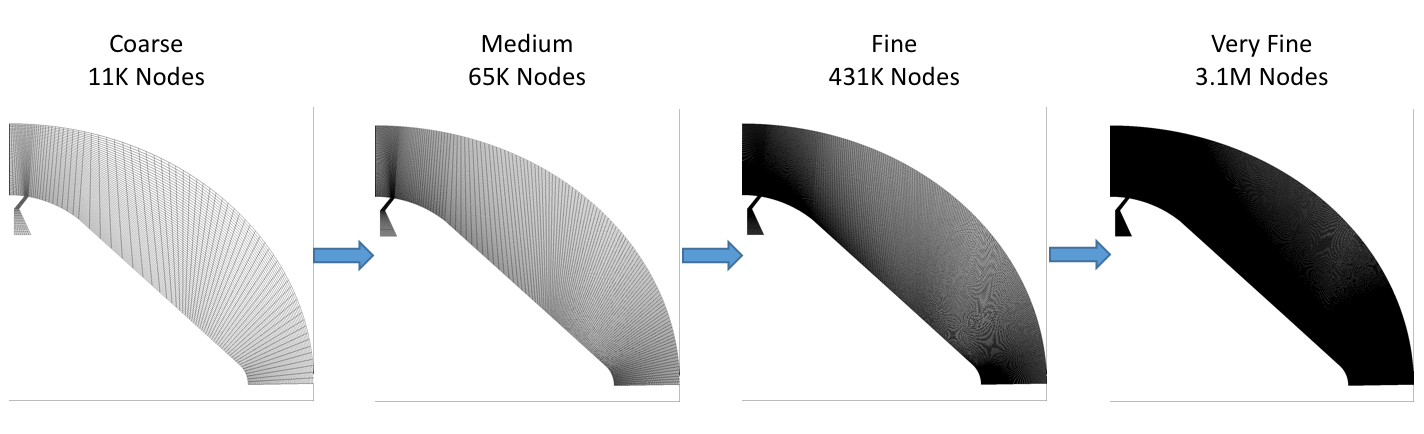
\includegraphics[width=\textwidth]{figures/mesh-progression.png}
  \end{figure}
  %------------------------------------------------------------------------------%
  \begin{itemize}
    \item Flow becomes unsteady as mesh is refined
    \item Very unsteady by finest grid level (3.1M Nodes)
    \item Solution is sensitive to flux limiter, regardless of mesh density
      \begin{itemize}
        \item Frozen flux limiter required by adjoint, and required ``tuning''
          Van Albada flux limiter to get consistent results
      \end{itemize}
  \end{itemize}
\end{frame}

\section{Design Optimization}
\stepcounter{subsection}
\subsection{Cost Function and Design Variables}

\begin{frame}
  \frametitle{Cost Function Definition}
  \begin{itemize}
    \item The optimization goal is to minimize a cost function generically
      defined as
  \end{itemize}
  \vspace{-0.1cm}
%------------------------------------------------------------------------------%
\begin{gather*}
  f = \sum_{j=1}^{N_{func}}w_j\left( C_j - C_{j^*} \right)^{p_j} \\
  \begin{aligned}
    C_j &= \text{Component value} \quad C_{j^*} &= \text{Component target} \\
    w_j &= \text{Component weight} \quad p_j &= \text{Component power}
  \end{aligned} \\
  N_{func} = \text{Number of cost function components}
\end{gather*}
%------------------------------------------------------------------------------%
\end{frame}

\begin{frame}
  \frametitle{Cost Function Integrated Areas}
  %------------------------------------------------------------------------------%
  \vspace{-0.8cm}
  \begin{figure}[h]
    \centering
    \subfloat[$T_{RMS}$ integrated area]{
      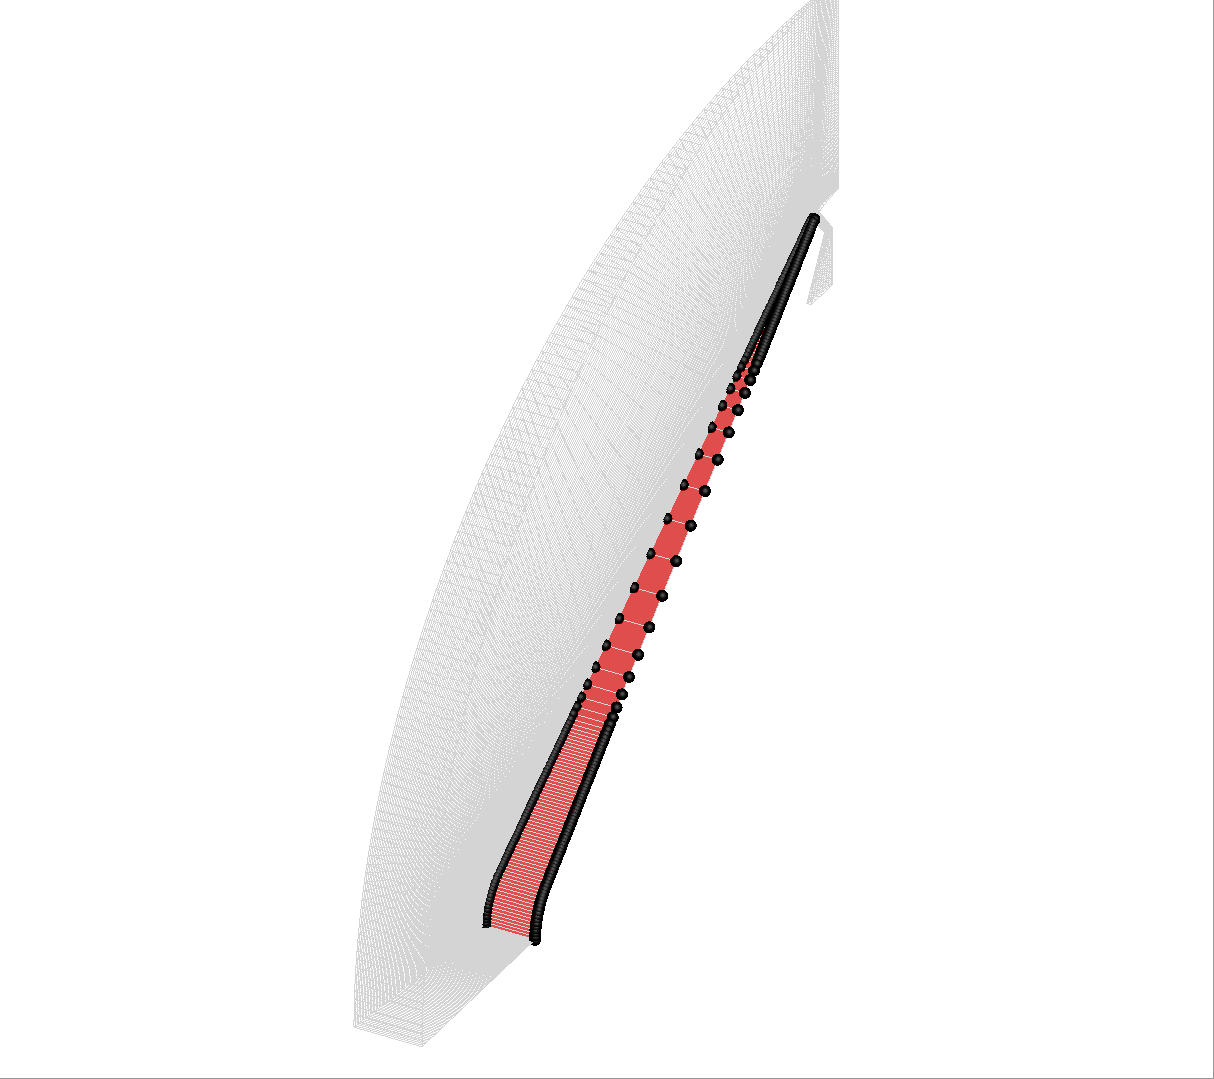
\includegraphics[width=0.35\textwidth]{figures/surface2.png}}
    \subfloat[$\massflow$ integrated area]{
      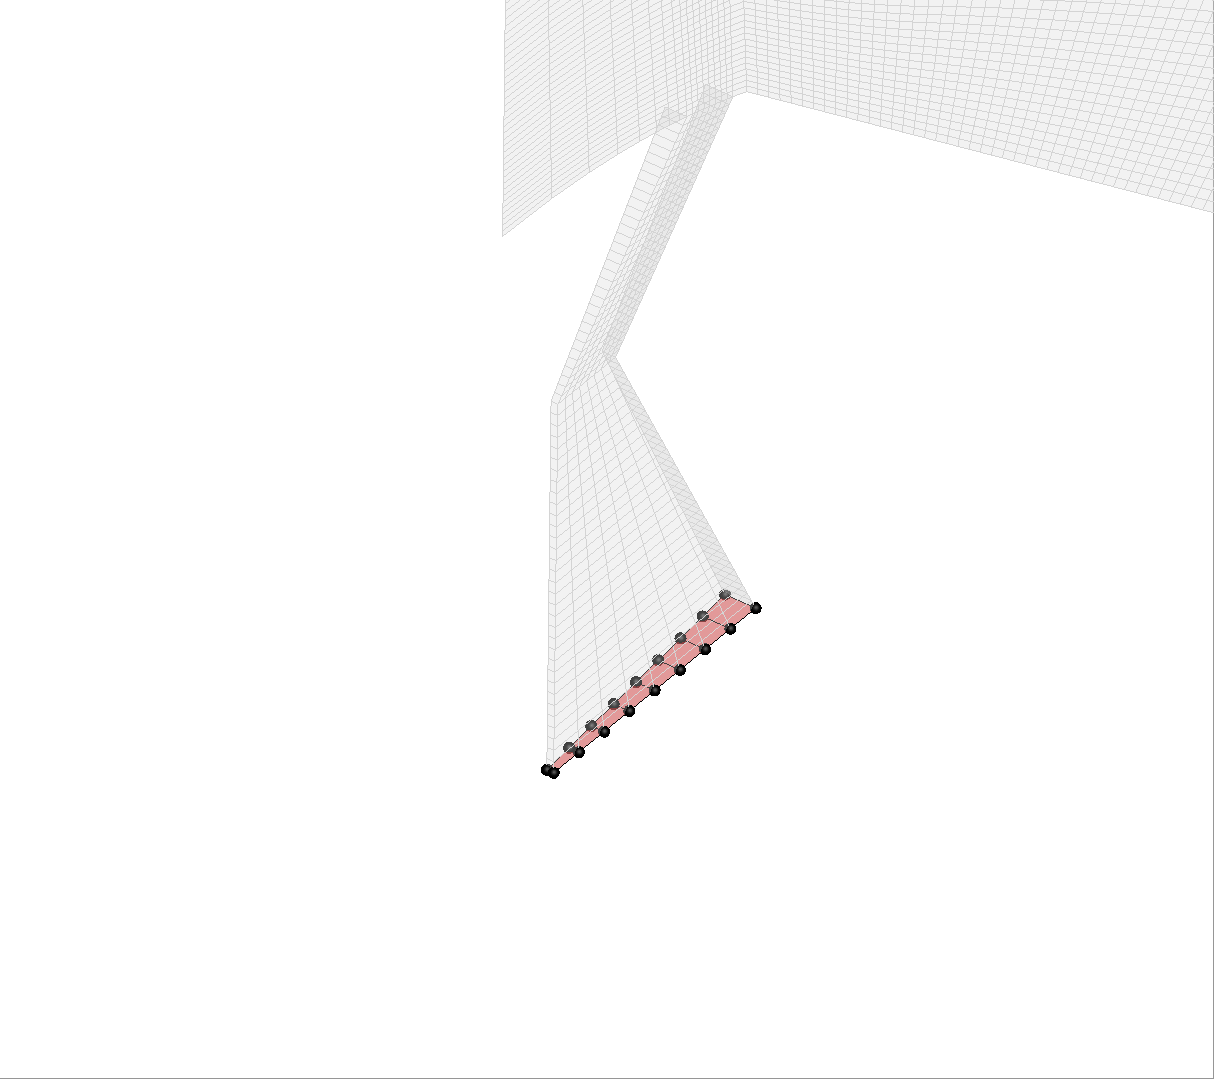
\includegraphics[width=0.35\textwidth]{figures/plenum_bc.png}}
  \end{figure}
  \vspace{-0.2cm}
  %------------------------------------------------------------------------------%
  \begin{itemize}
    \item Define cost function to minimize surface temperature RMS,
      $T_{RMS}$ and mass flow rate $\massflow$ through the annular plenum
%------------------------------------------------------------------------------%
      \[
        f = w_1\left( \massflow - \massflow^* \right)^2 
          + w_2\left( T_{RMS} - T_{RMS}^*\right)^2
      \]
%------------------------------------------------------------------------------%
  \end{itemize}
\end{frame}
\begin{frame}
  \frametitle{Design Variables}
  \begin{itemize}
    \item These plenum conditions are used as design variables:
      \begin{itemize}
        \item Plenum total pressure, $P_{p,o}$
        \item Plenum fuel-air ratio, $\fa$
      \end{itemize}
    \item The mass fractions of species $H_2$ and $N_2$ at the plenum are
      defined by the fuel-air ratio
%------------------------------------------------------------------------------%
\begin{equation*}
  \begin{aligned}
    c_{H_2} &= \fa \\
    c_{N_2} &= 1 - \fa
  \end{aligned}
\end{equation*}
%------------------------------------------------------------------------------%
  \item $\fa = 1$ corresponds to blowing pure $H_2$ from annular nozzle
  \item $\fa = 0$ corresponds to blowing pure $N_2$ from annular nozzle
  \end{itemize}
\end{frame}

\subsection{First-Order, Inverse Design Optimization}

\begin{frame}
  \frametitle{First-Order, Inverse Design Optimization}
  \begin{itemize}
    \item ``Inverse'' design optimization seeks to match a predetermined target
      design by altering a set of design inputs
    \item Sensitivity to frozen flux limiter mandated first-order for inverse
      design optimization
    \item Cost function with semi-arbitary targets specified
    \only<1>{
      \[
        f = w_1\cost{\massflow}^2
          + w_2\cost{T_{RMS}}^2
      \]
    }
    \only<2>{
      \[
        f = w_1\left( \massflow - 
        \begin{cboxf}[pink]
          \massflow^*
        \end{cboxf} \right)^2 
        + w_2\left( T_{RMS} - 
        \begin{cboxf}[blue]
          T_{RMS}^*
        \end{cboxf} \right)^2
      \]
    }
    \only<3>{
      \[
        f = w_1\left( \massflow - 
        \begin{cboxf}[pink]
          0.0024 
        \end{cboxf} \right)^2 
        + w_2\left( T_{RMS} - 
        \begin{cboxf}[blue]
          2000
        \end{cboxf} \right)^2
      \]
    }
    \item Weights chosen to normalize components for starting condition
      \[
        \frac{w_1}{w_2} = \frac{(T_{RMS} - 2000)^2}{(\massflow - 0.0024)^2}
      \]
  \end{itemize}
\end{frame}

\begin{frame}
  \frametitle{First-Order, Inverse Design Optimization}
  \only<1>{
  \begin{itemize}
    \item Target design is mostly met within 10 function evaluations
  \end{itemize}
  \vspace{-1cm}
%------------------------------------------------------------------------------%
\begin{figure}
  \centering
  \subfloat[Design variables]{
    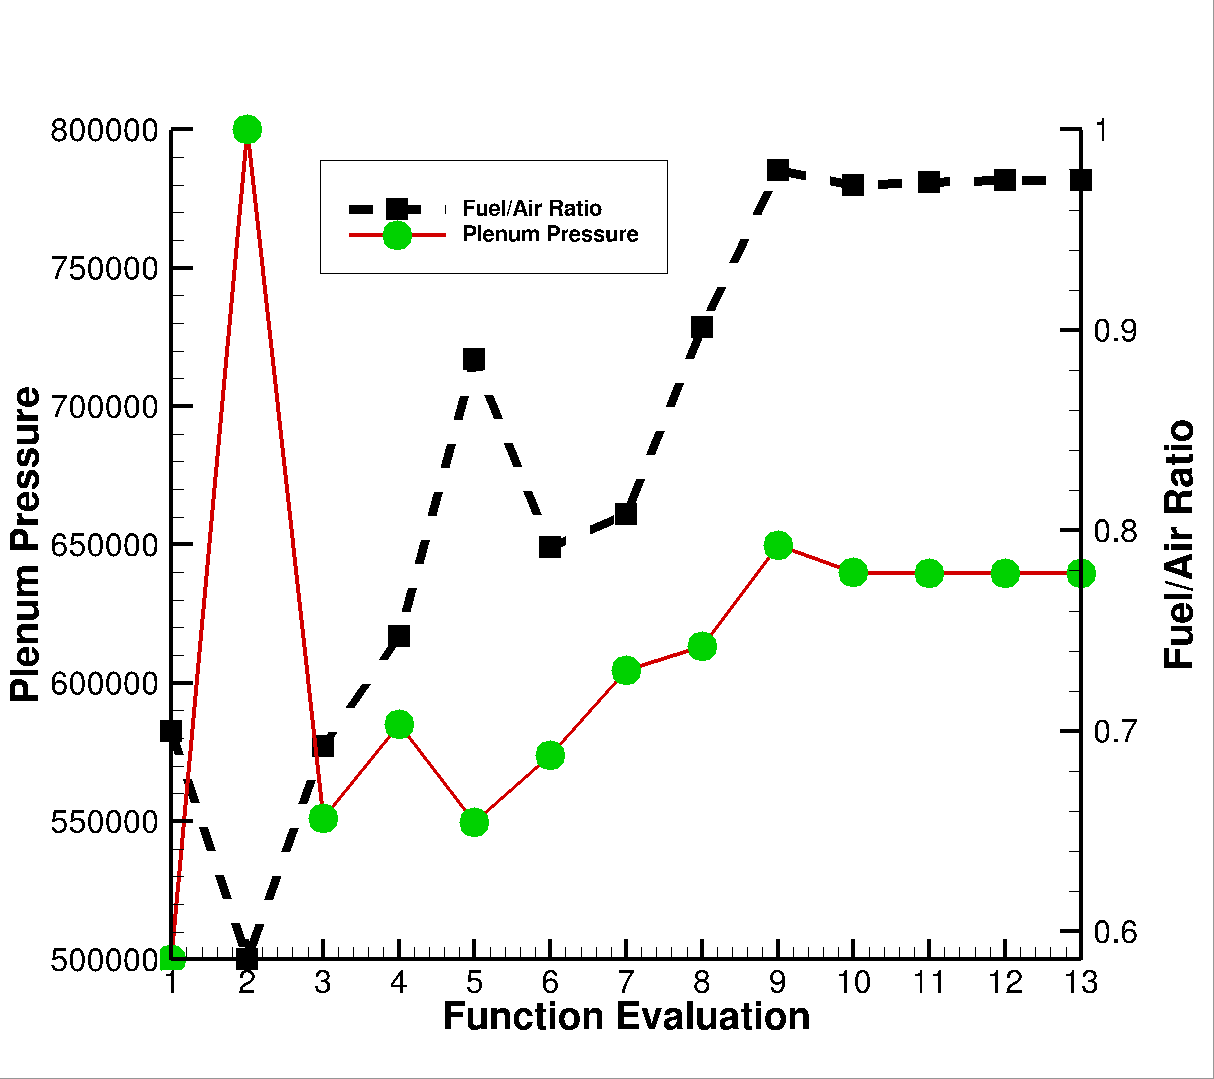
\includegraphics[width=0.5\textwidth]{figures/1st-H2/dv_hist.png}}
  \subfloat[Surface temperature RMS and mass flow rate]{
    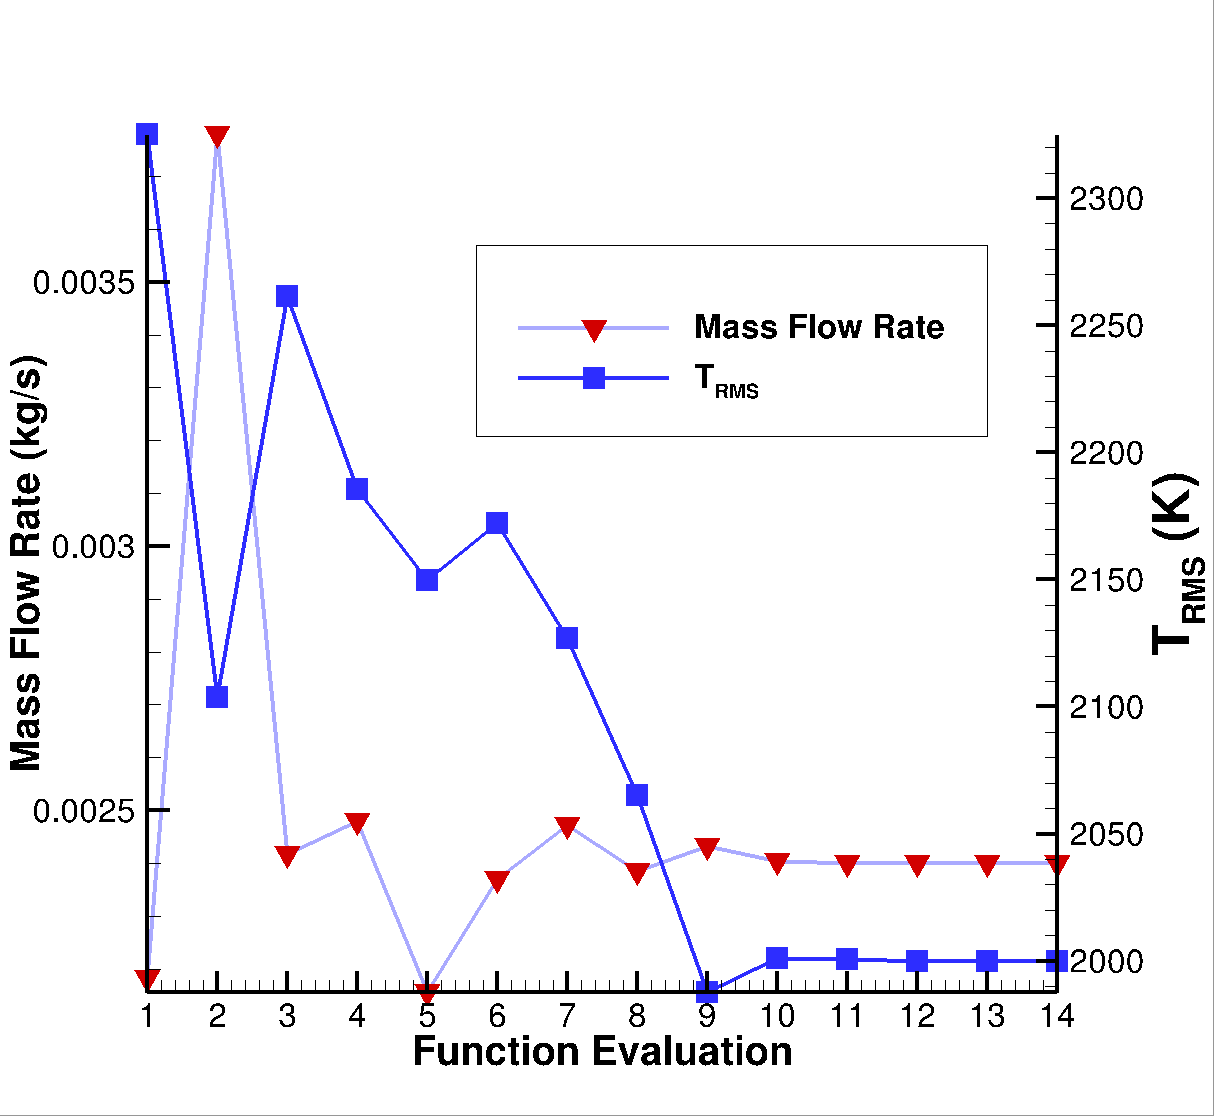
\includegraphics[width=0.5\textwidth]{figures/1st-H2/fm_hist.png}}
  \caption{Inverse design history}
\end{figure}
%------------------------------------------------------------------------------%
}
  \only<2>{
  \begin{itemize}
    \item Optimization terminated when cost function $< 10^{-8}$
    \item Cost function components are well normalized and approach zero as
      optimizer drives design to specified target
  \end{itemize}
  \vspace{-1cm}
%------------------------------------------------------------------------------%
\begin{figure}
  \centering
  \subfloat[Cost function value]{
    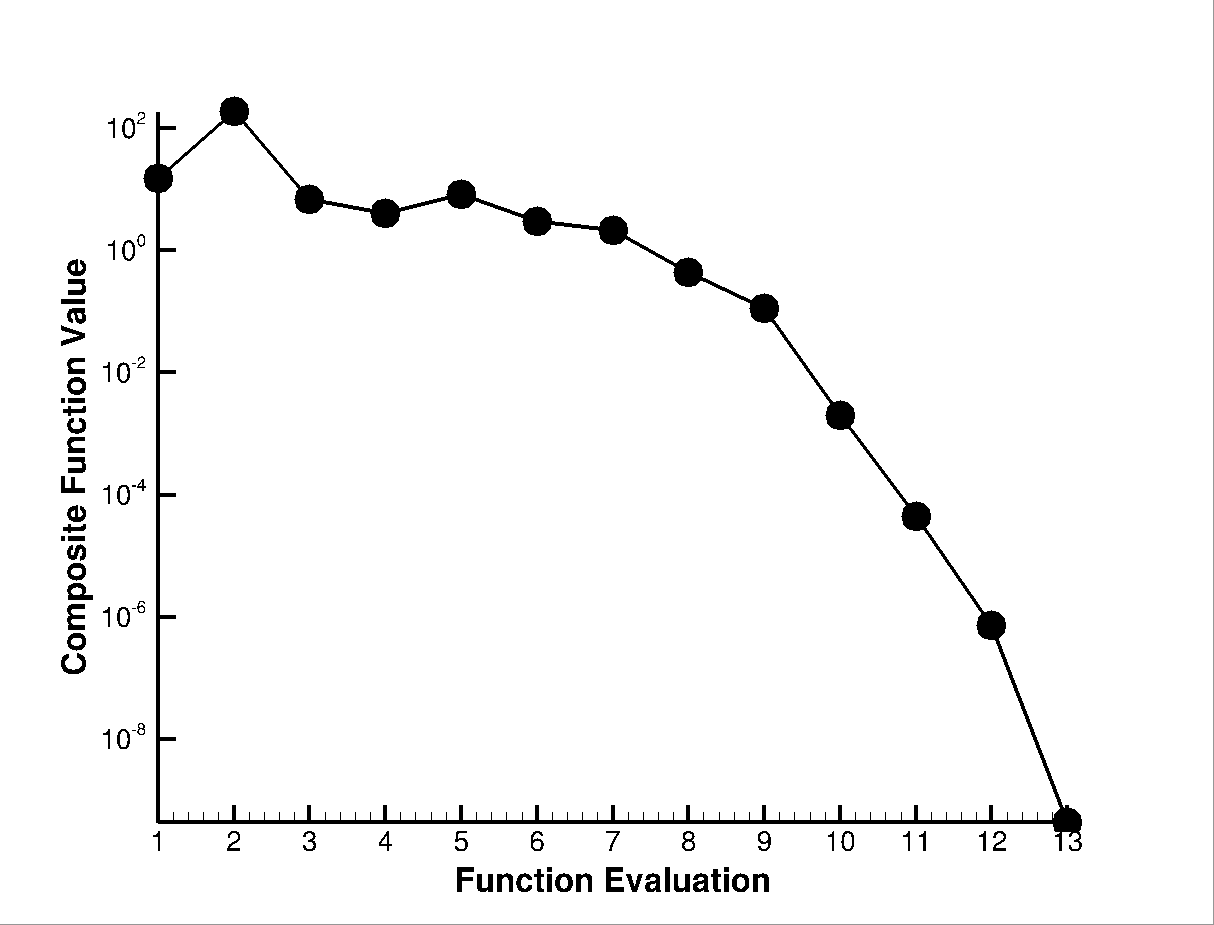
\includegraphics[width=0.5\textwidth]{figures/1st-H2/cost_func.png}}
  \subfloat[Component values]{
    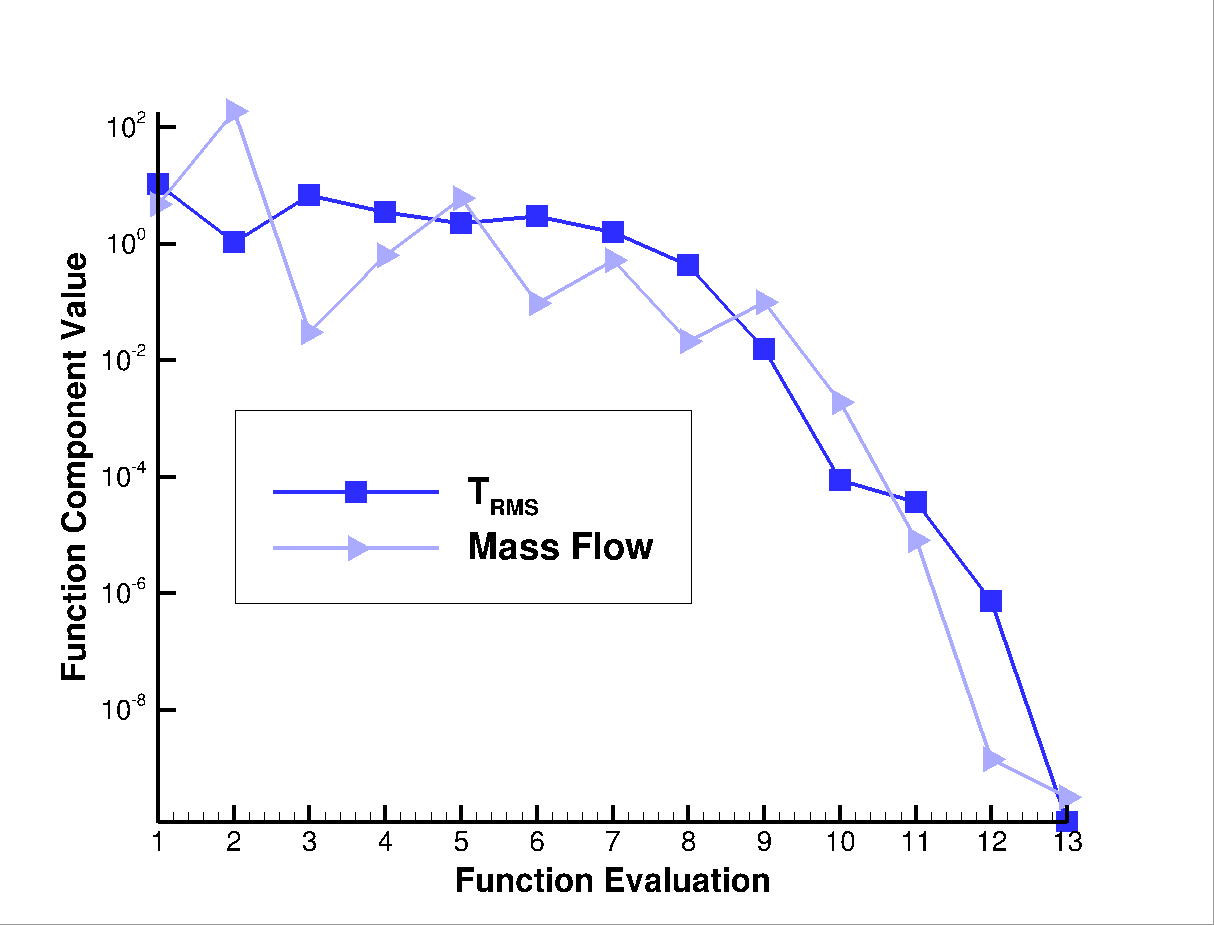
\includegraphics[width=0.5\textwidth]{figures/1st-H2/func_components.png}}
  \caption{Inverse design history}
\end{figure}
%------------------------------------------------------------------------------%
}
\end{frame}

\subsection{Second-Order, Direct Design Optimization}

\begin{frame}
  \frametitle{Second-Order, Direct Design Optimization}
  \begin{itemize}
    \item For direct optimization, the function is minimized with no
      predetermined target, so $T_{RMS}^*$ and $\massflow^*$ are set to zero
      \only<1>{
        \[
          f = w_1\left( \massflow - 
          \begin{cboxf}[pink]
            \massflow^*
          \end{cboxf} \right)^2 
          + w_2\left( T_{RMS} - 
          \begin{cboxf}[blue]
            T_{RMS}^*
          \end{cboxf} \right)^2
        \]
      }
      \only<2>{
        \[
          f = w_1\left( \massflow - 
          \begin{cboxf}[pink]
            \cancel{\massflow^*}
          \end{cboxf} \right)^2 
          + w_2\left( T_{RMS} - 
          \begin{cboxf}[blue]
            \cancel{T_{RMS}^*}
          \end{cboxf} \right)^2
        \]
      }
      \only<3>{
        \[
           f = w_1\left( \massflow \right)^2 
             + w_2\left( T_{RMS} \right)^2
        \]
      }
    \item Weights again chosen to normalize components based on starting design
      condition
      \[
        \frac{w_1}{w_2} = \frac{(T_{RMS})^2}{(\massflow)^2}
      \]
    \item This direct design optimization is much more sensitive to the choice of
      weights than the previous inverse design optimization
    \item Choice of weight can also be based on design requirements (i.e.
      preference to less mass over lower temperature)
  \end{itemize}
\end{frame}

\begin{frame}
  \frametitle{Second-Order, Direct Design Optimization}
  \only<1>{
  \begin{itemize}
    \item Design mostly driven by chemistry and $H_2$ lower molecular weight,
      relative to $N_2$
    \item The optimization is terminated after 9 function evaluations, when
      change in all design variables $<10^{-8}$
  \end{itemize}
  \vspace{-1.1cm}
%------------------------------------------------------------------------------%
\begin{figure}
  \centering
  \subfloat[Design variables]{
    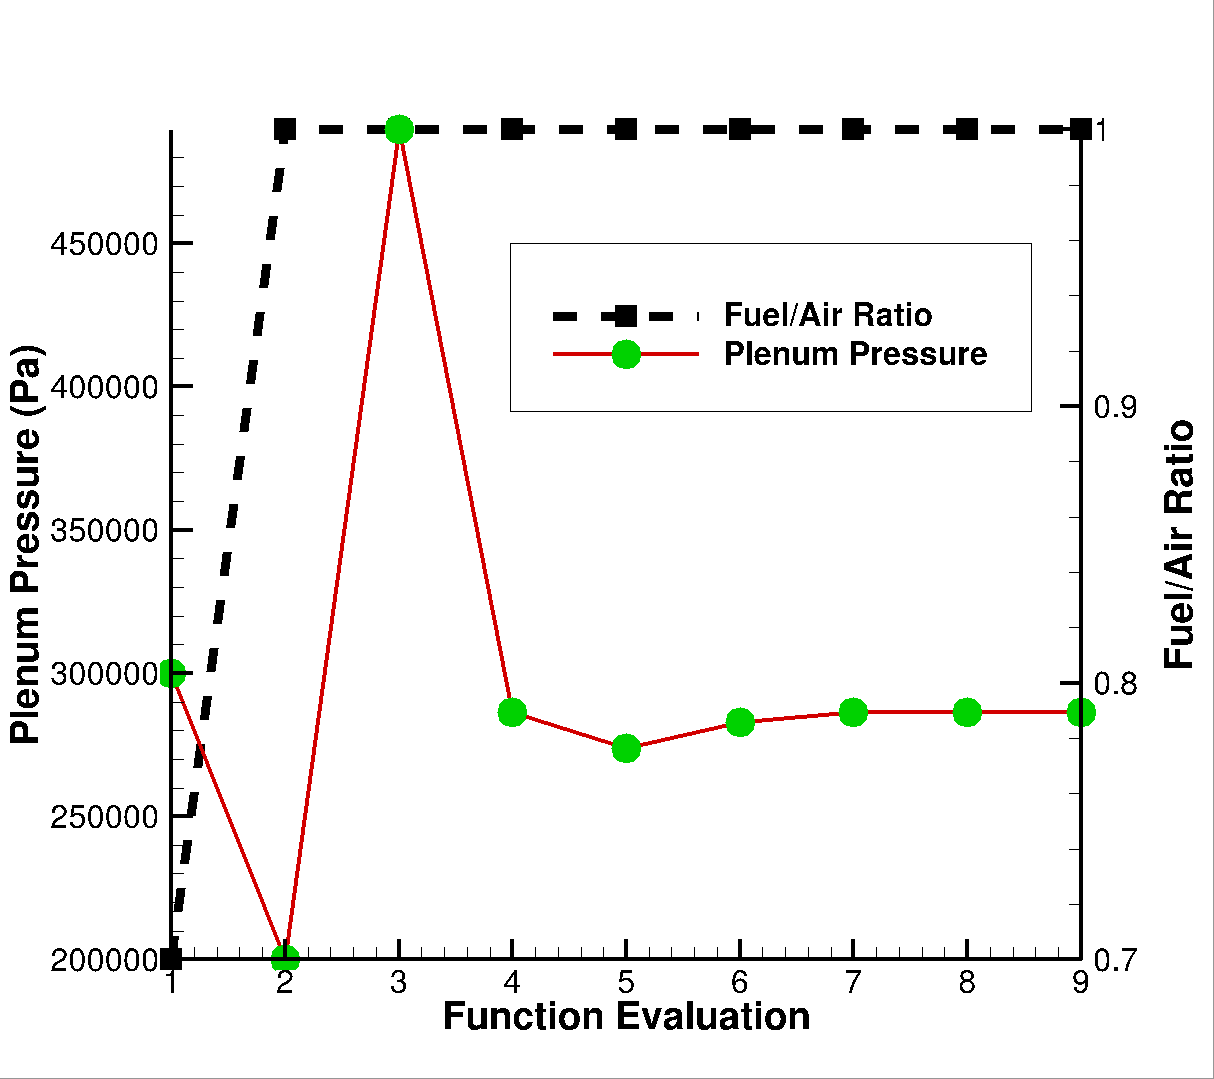
\includegraphics[width=0.5\textwidth]{figures/direct_design/dv-hist.png}}
  \subfloat[Surface temperature RMS and mass flow rate]{
    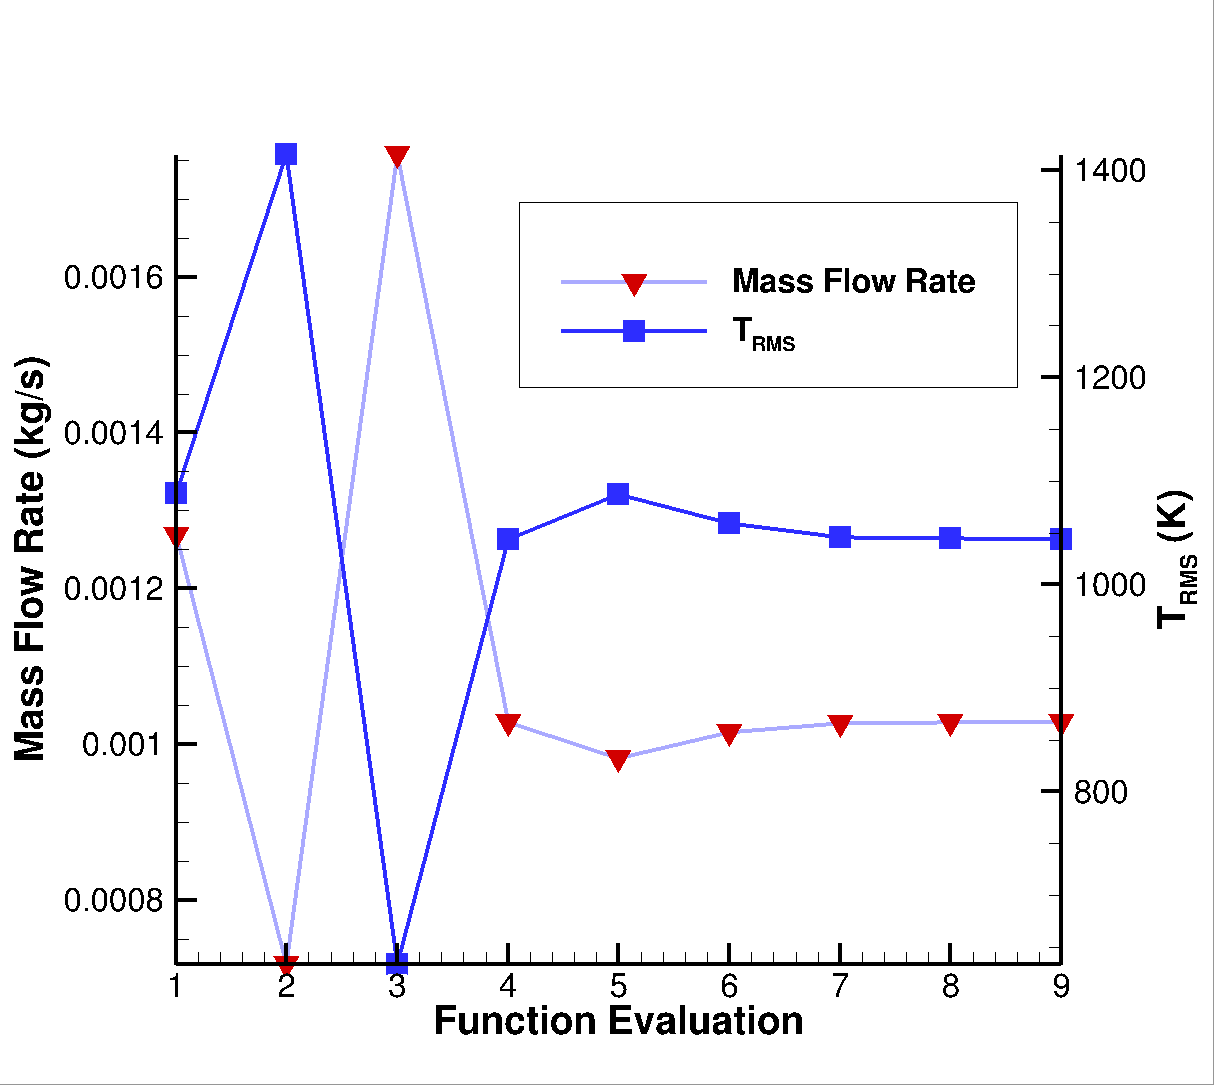
\includegraphics[width=0.5\textwidth]{figures/direct_design/mass-tt.png}}
  \caption{Direct design history}
\end{figure}
%------------------------------------------------------------------------------%
}
  \only<2>{
  \begin{itemize}
    \item Cost function components are well normalized
    \item Noticable net improvements stop after 4 function evaluations, due to
      weak dependence on plenum total pressure
  \end{itemize}
  \vspace{-1cm}
%------------------------------------------------------------------------------%
\begin{figure}
  \centering
  \subfloat[Cost function value]{
    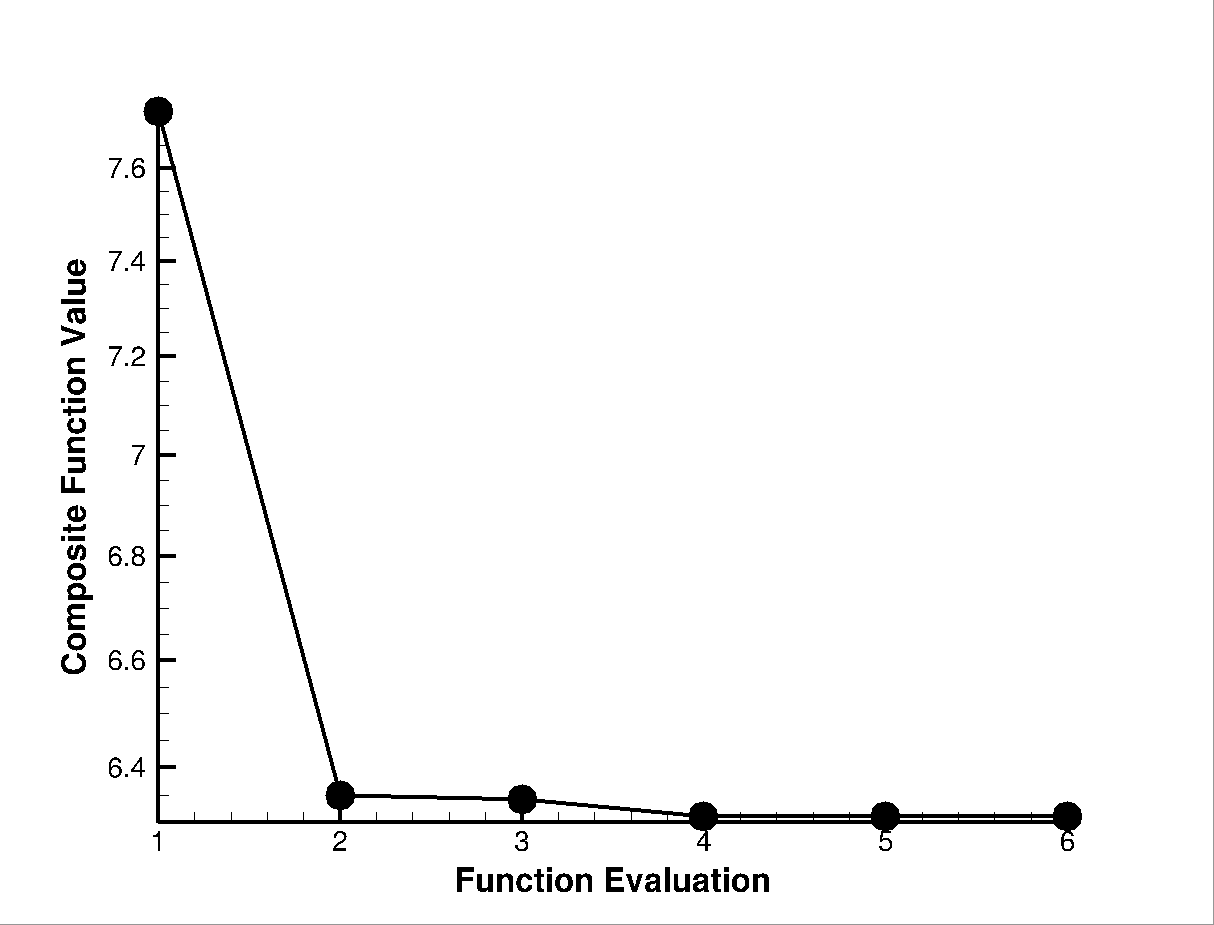
\includegraphics[width=0.5\textwidth]{figures/direct_design/cost-func.png}}
  \subfloat[Component values]{
    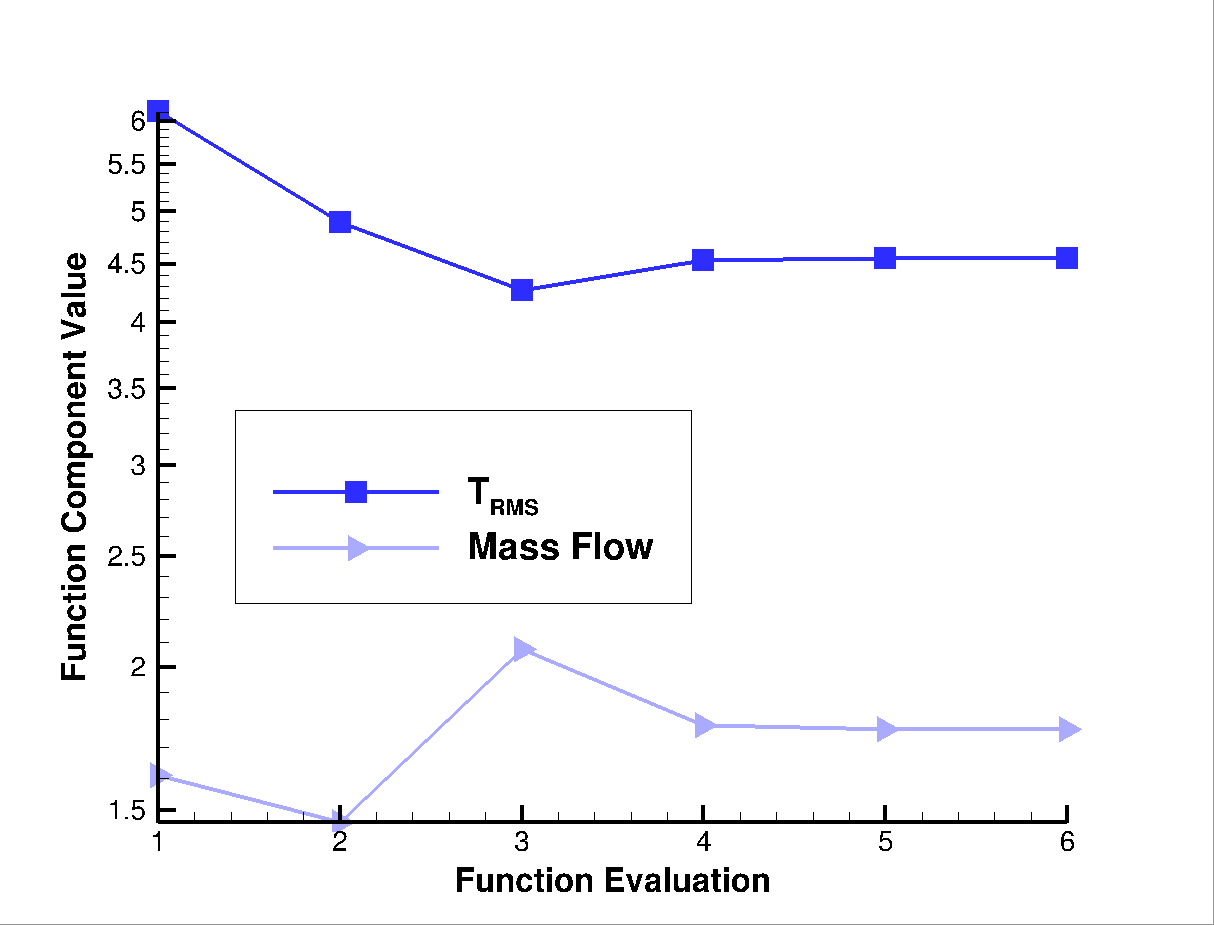
\includegraphics[width=0.5\textwidth]{figures/direct_design/components.png}}
  \caption{Direct design history}
\end{figure}
%------------------------------------------------------------------------------%
}
\end{frame}

\begin{frame}
  \frametitle{Second-Order, Direct Design Optimization}
%------------------------------------------------------------------------------%
\begin{table}[h]
  \small
  \centering
  \begin{tabular}{c|c|c|c}
    Component & Initial & Final & Improvement\\
    \hline
    $\dot{m}$, $kg/s$ & 1.268e-3 & 1.028e-3 & 18.93\% \\
    $T_{RMS}$, $K$    & 1088     & 1044     & 4.044\%
  \end{tabular}
  \caption{Direct design optimization improvement.}
  \label{tab:design-improvement}
\end{table}
%------------------------------------------------------------------------------%
\begin{itemize}
  \item Net $+22.9\%$ design improvement
  \item Optimizer significantly improved the mass flow rate, without largely
    affecting surface temperature
  \item Most gains associated with changing $\fa = 0.7 \rightarrow \fa = 1.0$
  \item Results can be tweaked by cost function component weighting
\end{itemize}

\end{frame}

\section{Accuracy and Relative Speedup}

\subsection{Accuracy and Consistency}

\begin{frame}
  \frametitle{Accuracy of the Adjoint Sensitivity Derivatives}
  \begin{itemize}
    \item To verify adjoint, derivatives computed by complex step eliminates
      subtractive cancellation error
%------------------------------------------------------------------------------%
    \[
      \pd{f}{x} = \frac{Im\left[ f(x + ih) \right]}{h} - O(h^2)
    \]
%------------------------------------------------------------------------------%
    \item Better agreement for frozen flow than chemically reacting flow
%------------------------------------------------------------------------------%
\begin{table}[h] 
  \tiny
  \centering 
  \begin{tabular}{c|c|c|c} 
    Design Variable & Adjoint & Complex & Relative Difference\\
    \hline 
    $P_{p,o}$ & -0.18451007644622E-06 & -0.184510076442032E-06 & 2.27e-11 \\ 
    $T_{p,o}$ &  0.62086963151678E-03 &  0.620869631517086E-03 & 4.93e-13 \\ 
    $\fa$     & -0.34045335117520E-01 & -0.340453351177196E-01 & 5.86e-12 
  \end{tabular}
  \caption{Sensitivity derivative comparison - $H_2$-$N_2$ frozen.}
  \label{tab:frozen-deriv-check}
\end{table}
\begin{table}[h]
  \centering
  \tiny
  \begin{tabular}{c|c|c|c}
    Design Variable & Adjoint & Complex & Relative Difference\\
    \hline
    $P_{p,o}$ & -0.11081315601976E-06 & -0.110529774659536E-06 & 2.56e-03 \\
    $T_{p,o}$ &  0.19089941237390E-03 &  0.190892847933810E-03 & 3.44e-05 \\
    $\fa$     & -0.28035409045530E-01 & -0.280251731728184E-01 & 3.65e-04
  \end{tabular}
  \caption{Sensitivity derivative comparison - $H_2$-$N_2$ reacting.}
  \label{tab:react-deriv-check}
\end{table}
%------------------------------------------------------------------------------%
  \end{itemize}
\end{frame}

\begin{frame}
  \frametitle{Accuracy of the Adjoint Sensitivity Derivatives}
  \begin{itemize}
    \item Difference is explained by relative convergence of frozen flow vs.
      flow with finite-rate chemistry
  %------------------------------------------------------------------------------%
  \begin{figure}
    \centering
    \adjincludegraphics[height=4.5cm,trim={0 0 0.5cm 4cm},clip]{figures/limiters/chem-res-comp.png}
  \end{figure}
  \vspace{-0.2cm}
  %------------------------------------------------------------------------------%
    \item Convergence of reacting flow stalls $\sim 8$ orders of magnitude
      before the convergence of frozen flow.
    \item This degrades the discrete comparison of adjoint and complex step
      derivatives, because many digits are still changing
  \end{itemize}
\end{frame}
\begin{frame}
  \frametitle{Consistency of Decoupled Solvers}
  \begin{itemize}
    \item Good agreement between decoupled and fully coupled flow solvers for
      temperature RMS and plenum mass flow rate
    %------------------------------------------------------------------------------%
    \begin{table}
      \tiny
      \centering
      \begin{tabular}{c|c|c|c}
        Quantity & Decoupled & Fully Coupled & Relative Difference \\
        \hline
        $\massflow$ & 0.8448720721551258E-03 & 0.8448720721551088E-03 & 2.01E-14 \\
        $T_{RMS}$   & 0.1545729169703027E+04 & 0.1545720949811712E+04 & 5.32E-06
      \end{tabular}
      \caption{Flow solution difference with finite-rate chemistry.}
    \end{table}
    %------------------------------------------------------------------------------%
    \item Very good agreement between the sensitivity derivatives computed by
      the decoupled and fully coupled adjoint solvers
%------------------------------------------------------------------------------%
\begin{table}[h]
  \tiny
  \centering
  \begin{tabular}{c|c|c|c}
    Design Variable & Decoupled Sensitivity & Fully Coupled Sensitivity & Rel. Diff\\
    \hline
    $P_{p,o}$ & -0.11081315601976E-06 & -0.11081315649260E-06 & 4E-9  \\
    $T_{p,o}$ &  0.19089941243495E-03 &  0.19089941237390E-03 & 3E-10 \\
    $\fa$     & -0.28035409093945E-01 & -0.28035409045530E-01 & 1E-9
  \end{tabular}
  \caption{Adjoint solution difference with finite-rate chemistry.}
\end{table}
%------------------------------------------------------------------------------%
  \end{itemize}
\end{frame}

\subsection{Relative Speedup of Decoupled Solvers}

\begin{frame}
  \frametitle{Relative Speedup of Decoupled Flow Solver}
  \vspace{-0.25cm}
  \begin{figure}[h]
    \centering
    \subfloat[Relative cost]{
      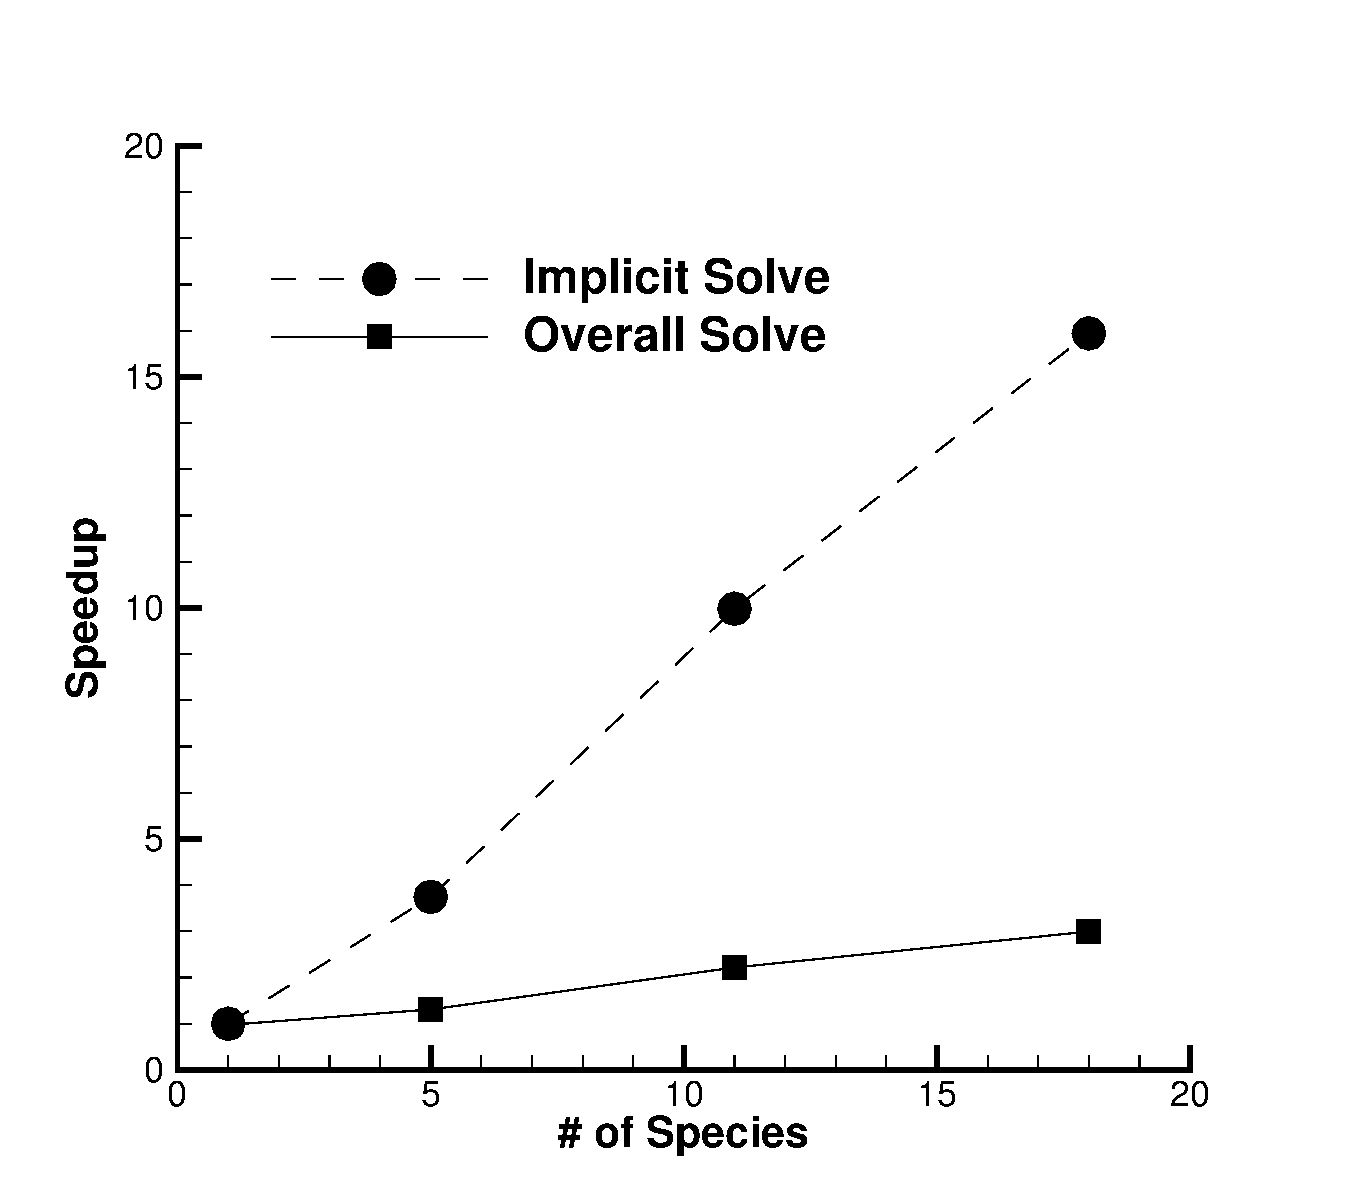
\includegraphics[width=0.45\textwidth]{figures/scitech/speedup}}
    \subfloat[Relative memory required]{
      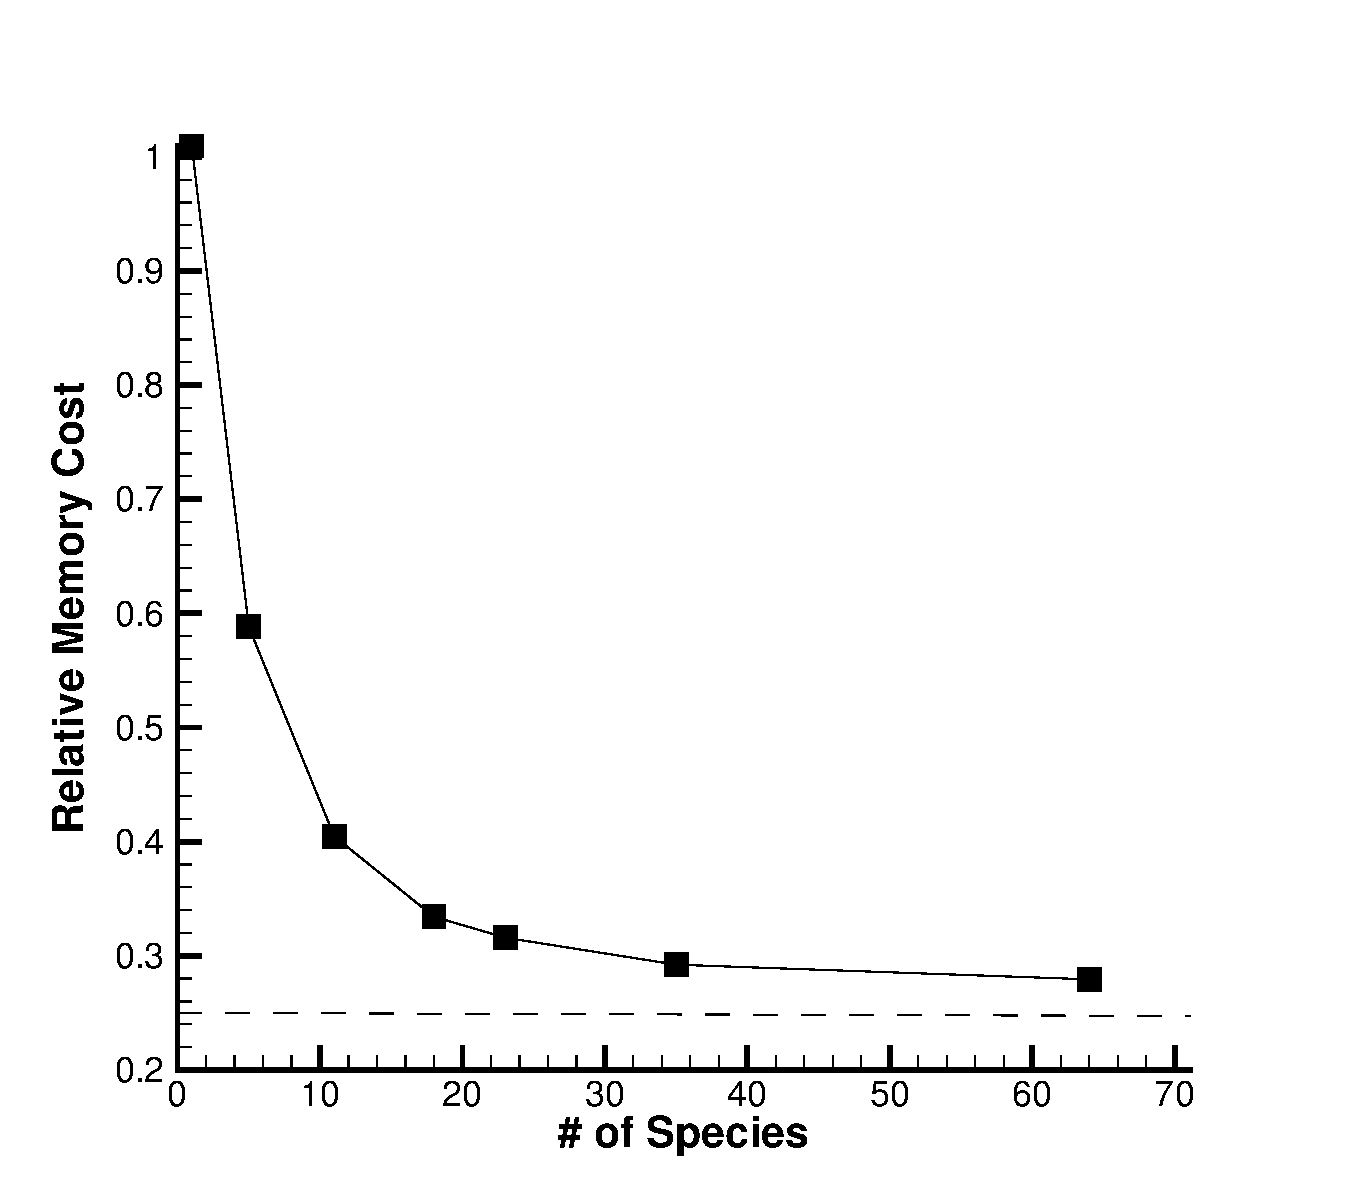
\includegraphics[width=0.45\textwidth]{figures/scitech/mem_req}}
  \end{figure}
  \begin{itemize}
    \item 5 $km/s$ Cylinder flow confirms that speedup in linear solver and
      overall solver increases linearly with number of species
    \item Relative memory required by the flow solver approaches $\sim 1/4$,
      which is correct when off-diagonal Jacobian elements are single precision
  \end{itemize}
\end{frame}

\begin{frame}
  \frametitle{Relative Speedup of Decoupled Flow Solver}
  \begin{itemize}
    \item For annular jet demonstration problem, speedup is much better for
      frozen flow, where convergence is clean
      \begin{itemize}
        \item More Jacobian evalutations are required due to stiffness of chemical
          source terms, which bottlenecks decoupled flow solver performance
      \end{itemize}
%------------------------------------------------------------------------------%
\begin{table}[h]
  \tiny
  \centering
  \begin{tabular}{c|c|c}
    Scheme & Time (s) & Speedup \\
    \hline
    Fully Coupled (Approximate) & 348.6 & 1.0 (baseline) \\
    Fully Coupled (Exact)       & 265.6 & 1.31 \\
    Decoupled                   & 138.7 & 2.51
  \end{tabular}
  \caption{Relative speedup for frozen chemistry.}
  \label{tab:srp-rel-speedup-frozen}
\end{table}
%------------------------------------------------------------------------------%
%------------------------------------------------------------------------------%
\begin{table}[h]
  \tiny
  \centering
  \begin{tabular}{c|c|c}
    Scheme & Time (s) & Speedup \\
    \hline
    Fully Coupled (Exact)       & 280.6 & 1.0 (baseline) \\
    Fully Coupled (Approximate) & 270.4 & 1.04 \\
    Decoupled                   & 168.6 & 1.66
  \end{tabular}
  \caption{Relative speedup for finite-rate chemistry.}
  \label{tab:srp-rel-speedup-chem}
\end{table}
%------------------------------------------------------------------------------%
  \end{itemize}
\end{frame}

\begin{frame}
  \frametitle{Relative Speedup of Decoupled Adjoint Solver}
  \begin{figure}[h]
    \centering
    \subfloat[Linearizations always recomputed]{
      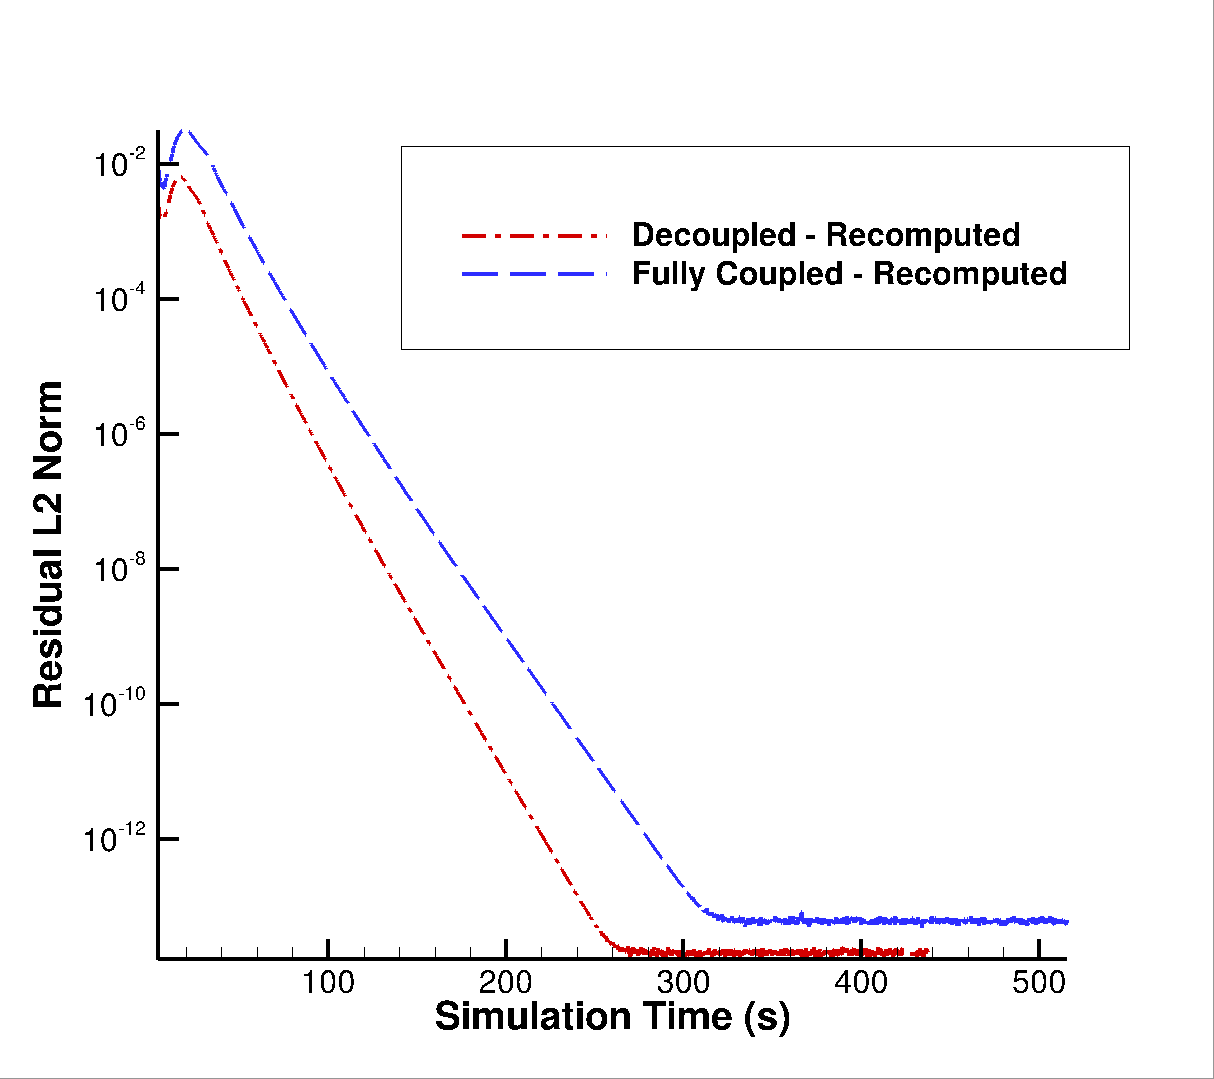
\includegraphics[width=0.45\textwidth]{figures/adj-efficiency/adj-recompute.png}}
    \subfloat[Linearizations stored]{
      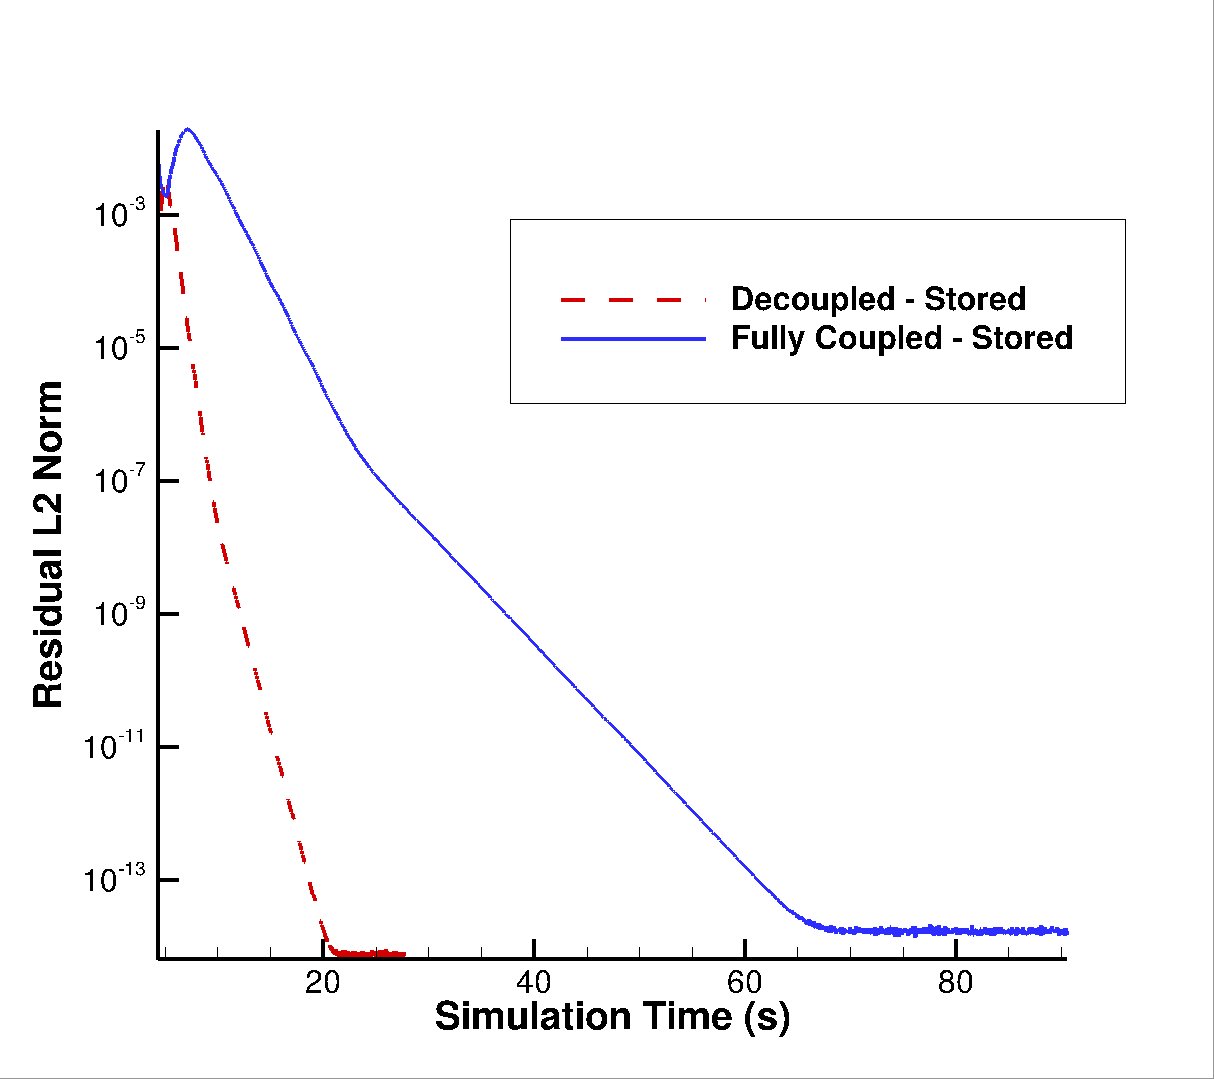
\includegraphics[width=0.45\textwidth]{figures/adj-efficiency/adj-stored.png}}
  \end{figure}
  \begin{itemize}
    \item Computing linearizations of second-order reconstruction is the
      dominant cost in the adjoint solve
      \begin{itemize}
        \item This can be mitigated by storing all linearizations, if there is
          enough memory
      \end{itemize}
  \end{itemize}
\end{frame}

\begin{frame}
  \frametitle{Relative Speedup of Decoupled Adjoint Solver}
  \vspace{-0.1cm}
  \begin{figure}[h]
    \centering
    \subfloat[Absolute memory required]{
      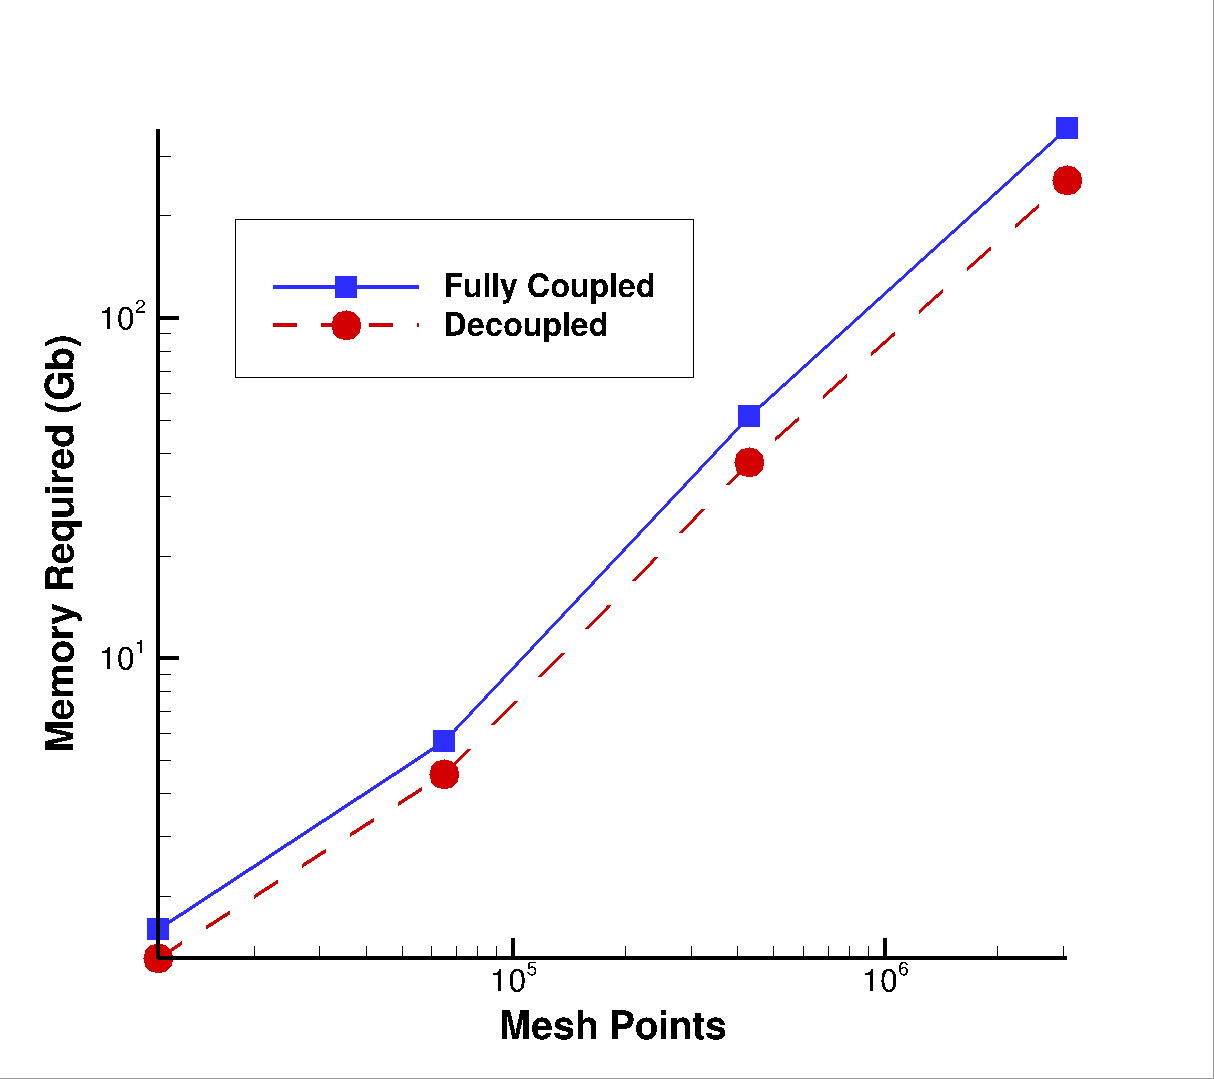
\includegraphics[width=0.4\textwidth]{figures/adj-efficiency/mem-req-srp.png}}
    \subfloat[Relative memory required]{
      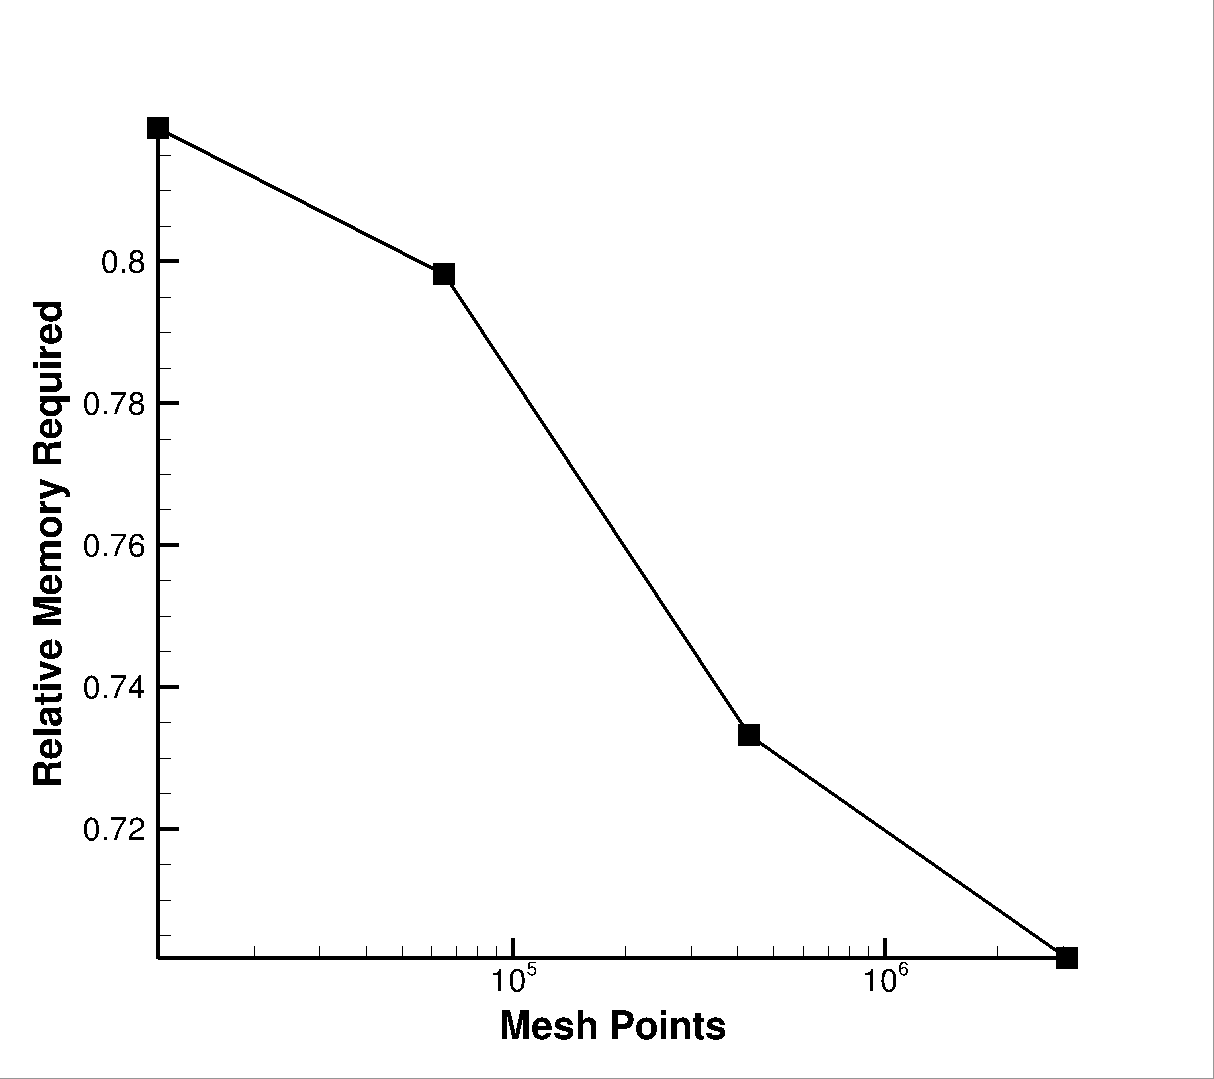
\includegraphics[width=0.4\textwidth]{figures/adj-efficiency/mem-rel-savings.png}}
    \caption{Memory required on annular jet meshes}
  \end{figure}
  \vspace{-0.2cm}
  \begin{itemize}
    \item Second-order Jacobian is much larger than first-order Jacobian used by
      flow solver
    \item Memory savings less than flow solver, but non-trivial ($\sim 20\%$)
    \item There are ways of trading CPUs for memory
  \end{itemize}
\end{frame}

\begin{frame}
  \frametitle{Relative Speedup of Decoupled Adjoint Solver}
\begin{itemize}
  \item Speedup in decoupled adjoint solver very beneficial if there is enough
    memory to store all linearizations
%------------------------------------------------------------------------------%
\begin{table}[h]
  \tiny
  \centering
  \begin{tabular}{c|c|c|c}
    Scheme & Linearizations & Time to Convergence (s) & Speedup \\
    \hline
    Fully Coupled & Recomputed  & 309.4 & 1.0 (baseline)\\
    Decoupled     & Recomputed  & 244.2 & 1.27 \\
    Fully Coupled & Stored      & 61.22 & 5.05 \\
    Decoupled     & Stored      & 18.69 & $\mathbf{16.6}$ \\
  \end{tabular}
  \caption{Relative speedup of decoupled to fully coupled adjoint solver.}
  \label{tab:srp-rel-speedup}
\end{table}
%------------------------------------------------------------------------------%
  \item Decoupled adjoint solver $\sim$ 3x faster than fully coupled adjoint
    solver if both store linearizations
  \item $16.6$x speedup is a credible scenario, due to decoupled scheme relative
    memory savings
\end{itemize}
\end{frame}

\section{Conclusion}
\stepcounter{subsection}

\begin{frame}
  \frametitle{Conclusion - Contributions}
  \begin{itemize}
    \item Contributions to the state of the art:
      \vspace{0.2cm}
      \begin{enumerate}
        \item<1-> Stable flow solver for inviscid flows in chemical
          non-equilibrium using a decoupled, point-implicit approach.
          \begin{itemize}
            \small
            \item Extended original derivation from Steger-Warming flux vector
              splitting method to Roe flux difference splitting method.
          \end{itemize}
          \vspace{0.2cm}
        \item<2-> Improved computational cost and memory required scaling with
          number of species continuity equations in adjoint solver.
          \begin{itemize}
            \small
            \item Order of magnitude speed increase if decoupled scheme memory
              savings enable linearization storage that was not possible with
              fully-coupled scheme
          \end{itemize}
          \vspace{0.2cm}
        \item<3-> Design optimization of a hypersonic reentry vehicle with a
          retro-firing annular jet.
          \begin{itemize}
            \small
            \item Direct and inverse design optimization on retro-propulsion
              case with challenging physics
          \end{itemize}
      \end{enumerate}
  \end{itemize}
\end{frame}

\begin{frame}
  \frametitle{Conclusion - Future Work}
  \begin{itemize}
    \item Extend decoupled flow solver and adjoint solver to viscous flows in
      thermal non-equilibrium
    \item Enable a mixed storage/recompute strategy for adjoint linearizations
    \item Expand the design variables possible for optimization
    \item Improve overall performance of FUN3D reacting gas path
  \end{itemize}
\end{frame}

\section{}

%\subsection{acknowledgements}

\begin{frame}
  \frametitle{Acknowledgements}
  \begin{itemize}
   \item Thanks to the FUN3D team at NASA Langley Research Center, for their
     support in integrating aspects of the compressible gas path into the
     reacting gas path of FUN3D.
   \item Thanks to Jeff White of the Computational Aerosciences Branch at NASA
     Langley Research Center, for his advice regarding reacting flow simulation.
   \item Thanks to Boris Diskin of the National Institute of Aerospace, for his
     advice on adjoint solvers.
   \item Thanks to the Entry Systems Modeling Project within the NASA
     Game Changing Development Program for their funding and support of this research.  
  \end{itemize}
\end{frame}
\begin{frame}
  \huge
  \centering
  {\bf Questions?}
\end{frame}
%\subsection{backup}

\begin{frame}
  \frametitle{Decoupled Point Implicit Flow Solver}
  \begin{itemize}
    \item The fluxes are solved in two sequential steps
      \begin{itemize}
        \item  The mixture fluxes are first solved as
        \[
          \frac{\partial \mU'}{\partial t} +
          \frac{1}{\vol}\sum\limits_{f}(\vF'\cdot\Norm)^f = 0
        \]
      \item Followed by the species fluxes
      \[
        \frac{\partial \mathbf{\hat{U}}}{\partial t} +
        \frac{1}{\vol}\sum\limits_{f}(\mathbf{\hat{F}}\cdot \Norm)^f =
        \mathbf{\hat{W}}
      \]
    \end{itemize}
    \item Since the mixture density was determined in the first step, step two
      actually solves for the species mass fractions
      \begin{gather*}
        \delta \mathbf{\hat{U}}^n 
        = \rho^{n+1} \hat{\mv}^{n+1}-\rho^n\mathbf{\hat{V}}^n = \rho^{n+1} \delta
        \mathbf{\hat{V}}^n + \mathbf{\hat{V}}^n \delta \rho^n \\
        \mathbf{\hat{V}}=(c_1,\hdots,c_{ns})^T, c_s=\rho_s/\rho
      \end{gather*}
  \end{itemize}
\end{frame}
\begin{frame}
  \frametitle{Decoupled Point Implicit Flow Solver}
  \vspace{-0.2cm}
  \begin{itemize}
    \item Chemical source term linearized via
    \vspace{-0.1cm}
    \begin{align*}
      \mathbf{\hat{W}}^{n+1} &= \mathbf{\hat{W}}^n+\frac{\partial
      \mathbf{\hat{W}}}{\partial \mathbf{U}}\bigg|_{\mathbf{U}'} \frac{\partial
      \mathbf{U}}{\partial \mathbf{\hat{V}}} \\
       \mc &= \frac{\partial \mathbf{\hat{W}}}{\partial
       \mathbf{U}}\bigg|_{\mathbf{U}'} \frac{\partial \mathbf{U}}{\partial
       \mathbf{\hat{V}}}
    \end{align*}
    \item Full system to be solved in step two
    \begin{sequation}[0.9]
      \begin{gathered}
        \frac{\vol}{\delta t} \rho^{n+1} \delta\Vhat + 
        \lsum{f}{}{ \left( 
          \pd{\Fhat^f}{\Vhat^L} \cdot \Norm^f \delta \Vhat^L 
        + \pd{\Fhat^f}{\Vhat^R} \cdot \Norm^f \delta \Vhat^R 
        \right)^{n,n+1}} 
        - \vol C^{n,n+1} \delta \Vhat^n \\ 
        = -\lsum{f}{}{
          \left( \Fhat^{n,n+1} \cdot \Norm \right)^f 
        } 
        + (\vol)(\omega_r)(\mw^{n, n+1}) + R_\rho \Vhat^n \\
        R_\rho =
        \lsum{f}{}{\lsum{s=1}{N_s}{(\hat{F}_{\rho_s}^{n,n+1}\cdot\mathbf{N})}} 
      \end{gathered}
    \end{sequation}
  \item $R_\rho$ is included to preserve $\sum\limits_{s}{c_s}=1$, $\sum\limits_{s}{\delta c_s}=0$.
  \end{itemize}
\end{frame}
\begin{frame}
  \frametitle{Geometry and Test Conditions}
  \begin{columns}
    \begin{column}{0.4\textwidth}
    %------------------------------------------------------------------------------%
      \vspace{-0.5cm}
    \begin{figure}
      \centering
      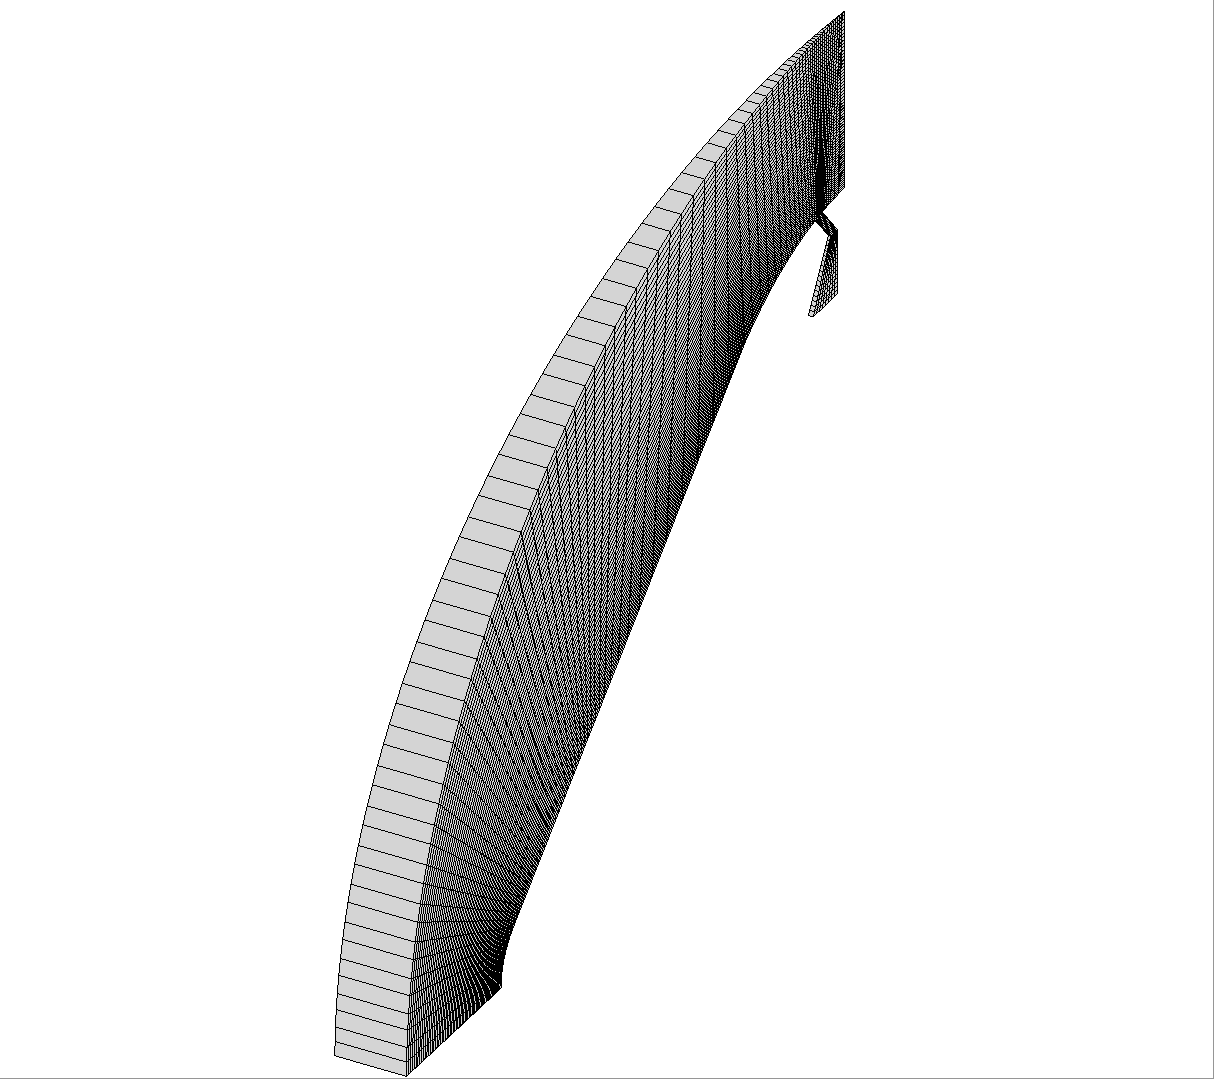
\includegraphics[width=0.7\textwidth]{figures/iso-coarse.png}
    \end{figure}
    \vspace{-0.75cm}
    \begin{figure}
      \centering
        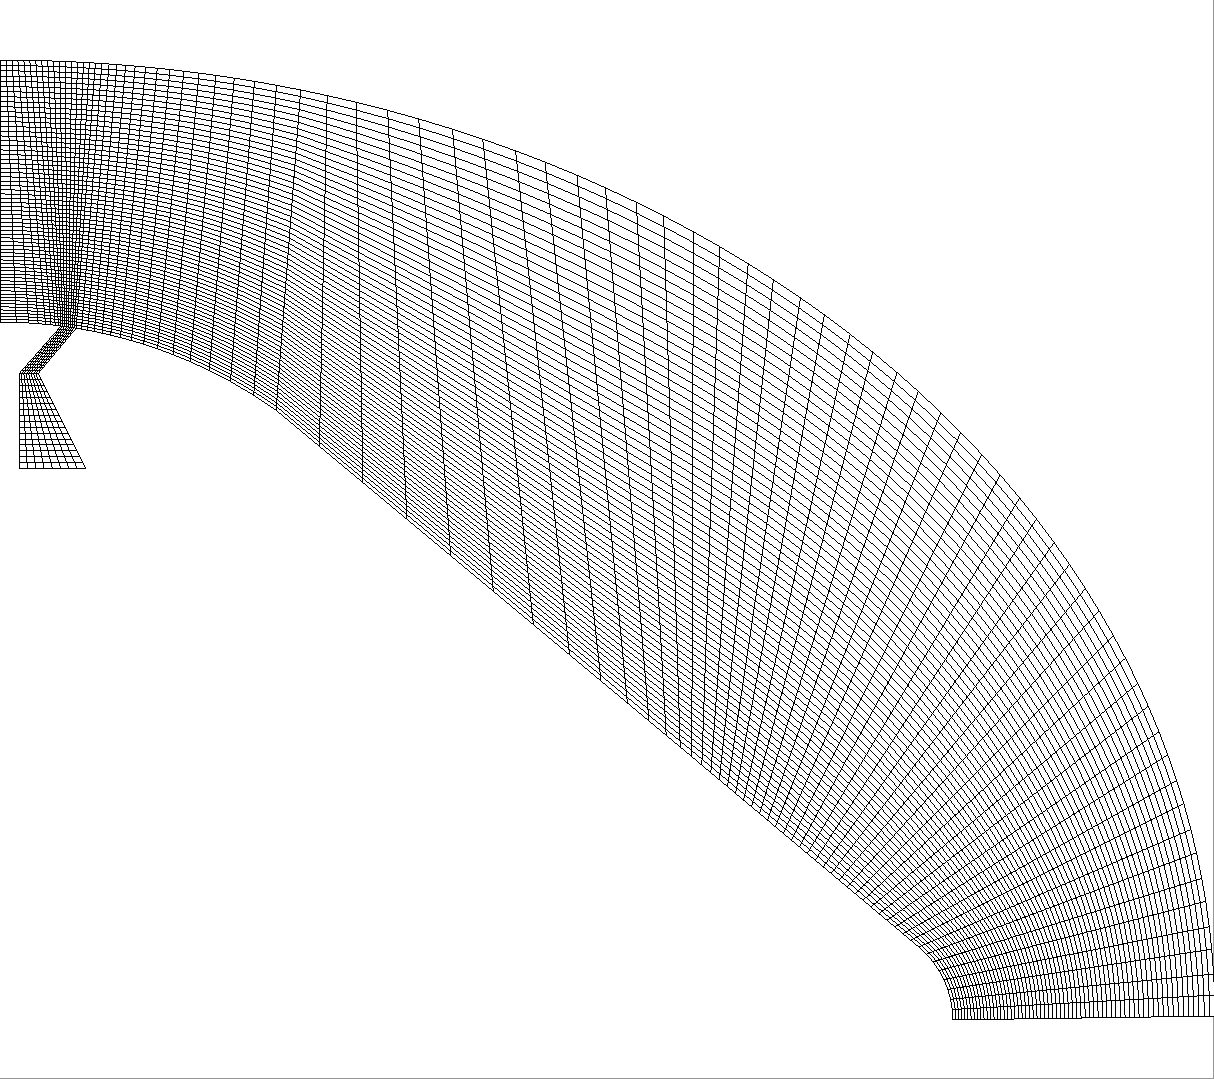
\includegraphics[width=\textwidth]{figures/side-coarse.png}
      \caption{Annular jet geometry.}
    \end{figure}
    %------------------------------------------------------------------------------%
    \end{column}
    \begin{column}{0.65\textwidth}
      \tiny
    %------------------------------------------------------------------------------%
    \begin{table}[h]
      \centering
      \begin{tabular}{c|c|c}
        Parameter & Description & Value \\
        \hline
        $r_{throat}$       &   nozzle throat radius, $m$                 & 0.02 \\
        $r_{plenum,inner}$ &   inside nozzle radius at plenum face, $m$  & 0.02 \\
        $r_{plenum,outer}$ &   outside nozzle radius at plenum face, $m$ & 0.07 \\
        $r_{exit,inner}$   &   inside nozzle radius at exit, $m$         & 0.064 \\
        $r_{exit,outer}$   &   outside nozzle radius at exit, $m$        & 0.08 \\
        $l_{conv}$         &   distance from plenum to throat, $m$       & 0.05 \\
        $\theta_c$         &   cone half angle, deg                      & 50.0
      \end{tabular}
      \caption{Annular nozzle geometry inputs.}
      \label{tab:annular-geom}
    \end{table}
    %------------------------------------------------------------------------------%
    %------------------------------------------------------------------------------%
    \begin{table}[!h]
      \centering
      \begin{tabular}{c|c|c}
        Flow Condition & Description & Value \\
        \hline
        $V_{\infty}$    & freestream velocity, $m/s$        & 5686.24 \\
        $\rho_{\infty}$ & freestream density, $kg/m^3$      & 0.001 \\
        $T_{\infty}$    & freestream temperature, $K$       & 200.0 \\
        $M_{\infty}$    & freestream Mach number (derived)  & 20.0
      \end{tabular}
      \caption{Flow conditions.}
      \label{tab:flow-conditions-backup}
    \end{table}
    %------------------------------------------------------------------------------%
    \end{column}
  \end{columns}
\end{frame}
\begin{frame}
  \frametitle{Flux Limiter Sensitivity}
  \begin{itemize}
    \item First-order and second-order solutions very different, so
      choice of flux limiter has strong impact on steady state solution
    \item Van Albada with tuneable parameter, $\varepsilon = 0.01$, least
      sensitive to ``freezing'' the limiter
  \end{itemize}
  \vspace{-0.5cm}
%------------------------------------------------------------------------------%
\begin{figure}[h]
  \centering
  \subfloat{
    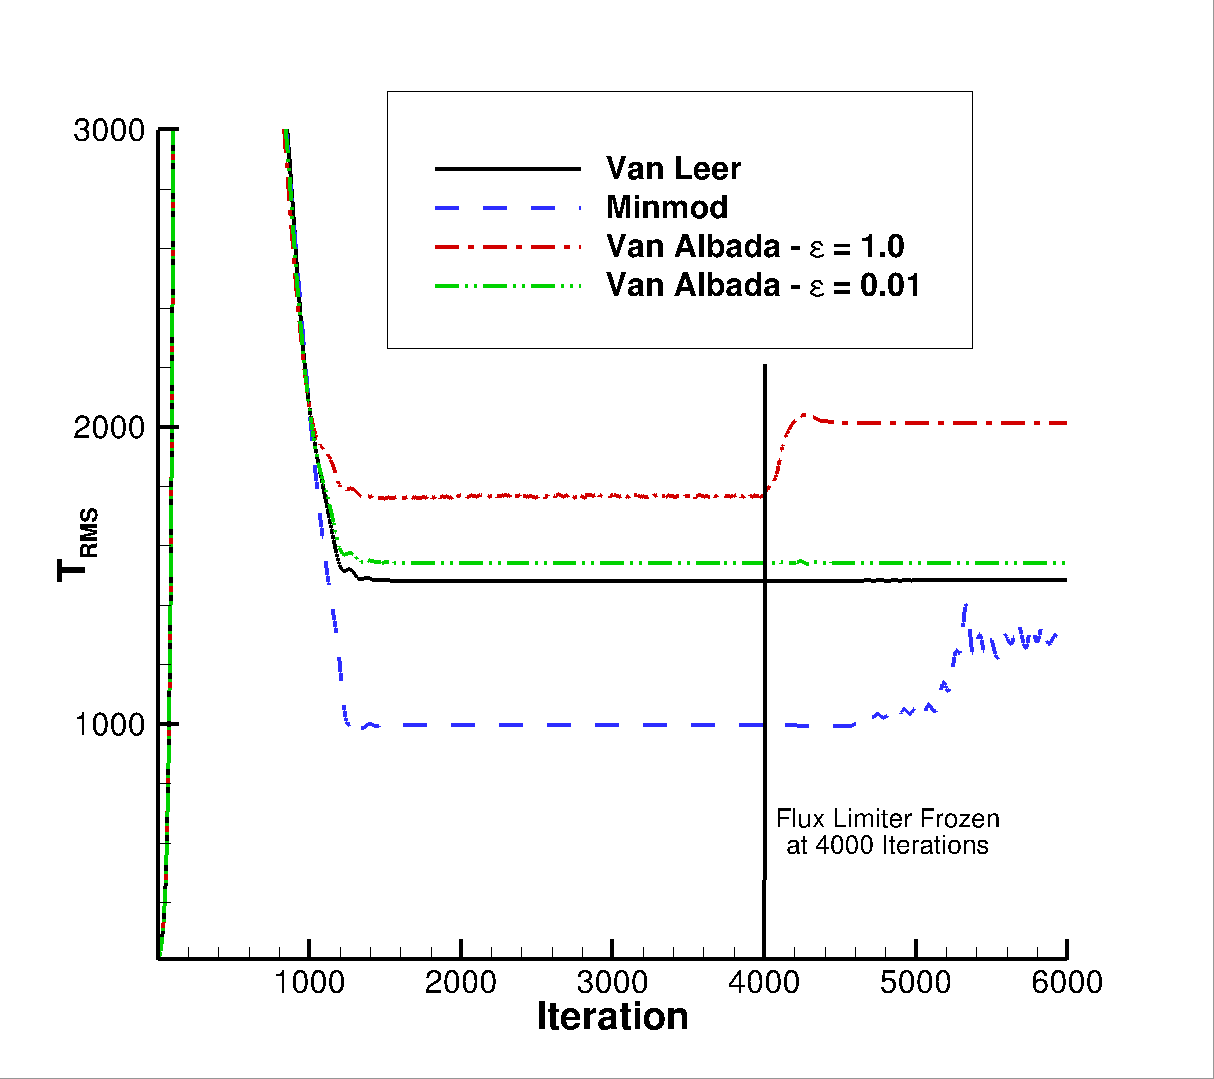
\includegraphics[width=0.45\textwidth]{figures/limiters/all-limiters.png}}
  \subfloat{
    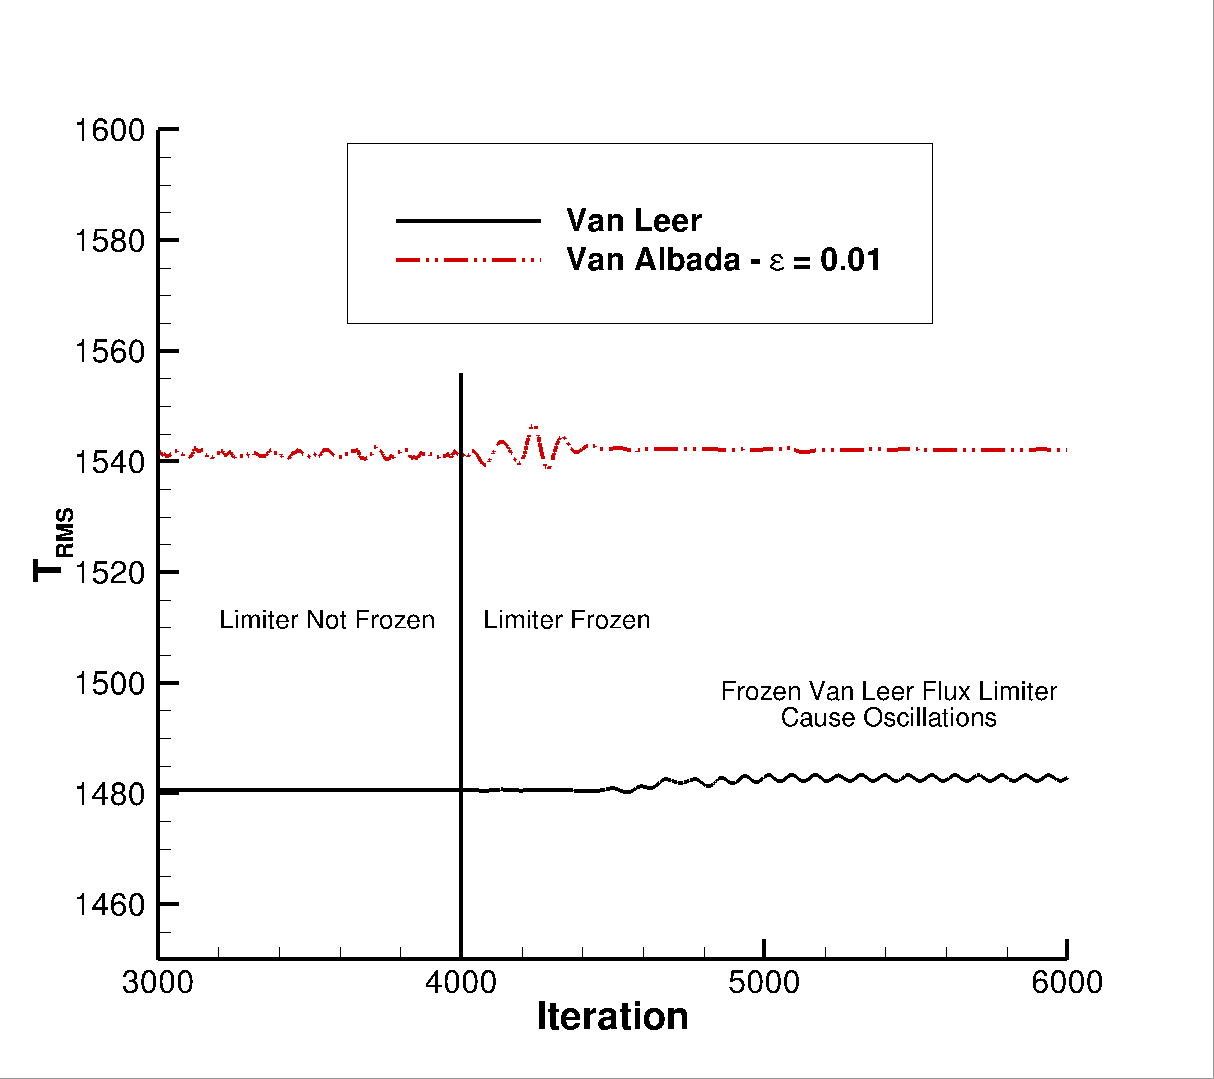
\includegraphics[width=0.45\textwidth]{figures/limiters/vanleer-vanalbada-frozen.png}}
  \caption{Flux limiter impact on surface temperature.}
  \label{fig:vl-va-impact}
\end{figure}
%------------------------------------------------------------------------------%
\end{frame}
\begin{frame}
  \frametitle{Mesh Refinement Study}
%------------------------------------------------------------------------------%
\begin{figure}[h]
  \centering
  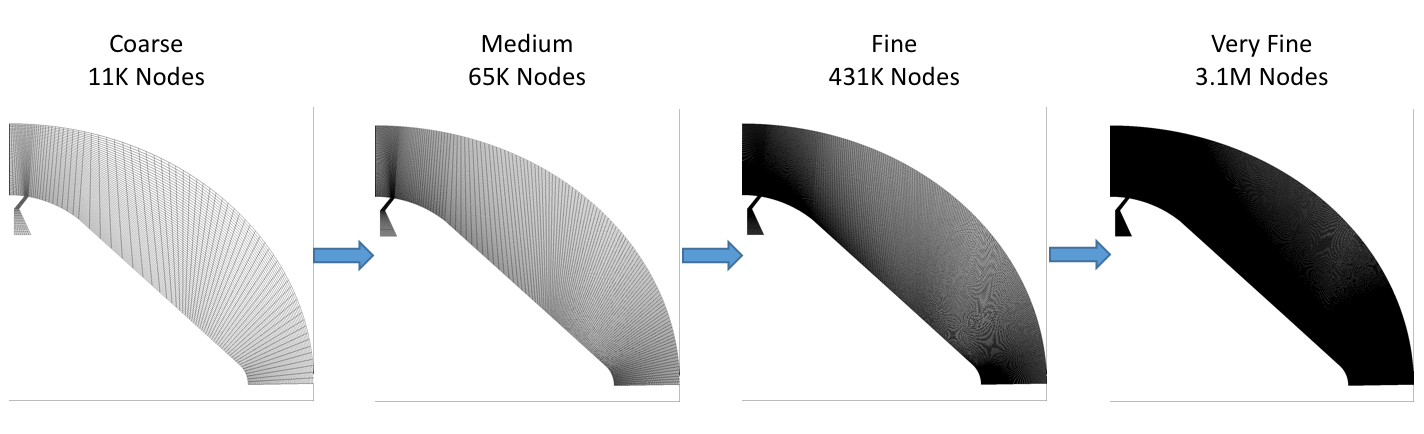
\includegraphics[width=0.75\textwidth]{figures/mesh-progression.png}
\end{figure}
\vspace{-1cm}
%------------------------------------------------------------------------------%
  \begin{columns}
    \begin{column}{0.5\textwidth}
      \begin{itemize}
        \item Flow becomes unsteady as mesh is refined
        \item Very unsteady by finest grid level (3.1M Nodes)
        \item Coarse mesh used in optimization still retains all of the
          challenging physics of the problem
      \end{itemize}
    \end{column}
    \begin{column}{0.5\textwidth}
%------------------------------------------------------------------------------%
\begin{figure}[!h]
  \centering
  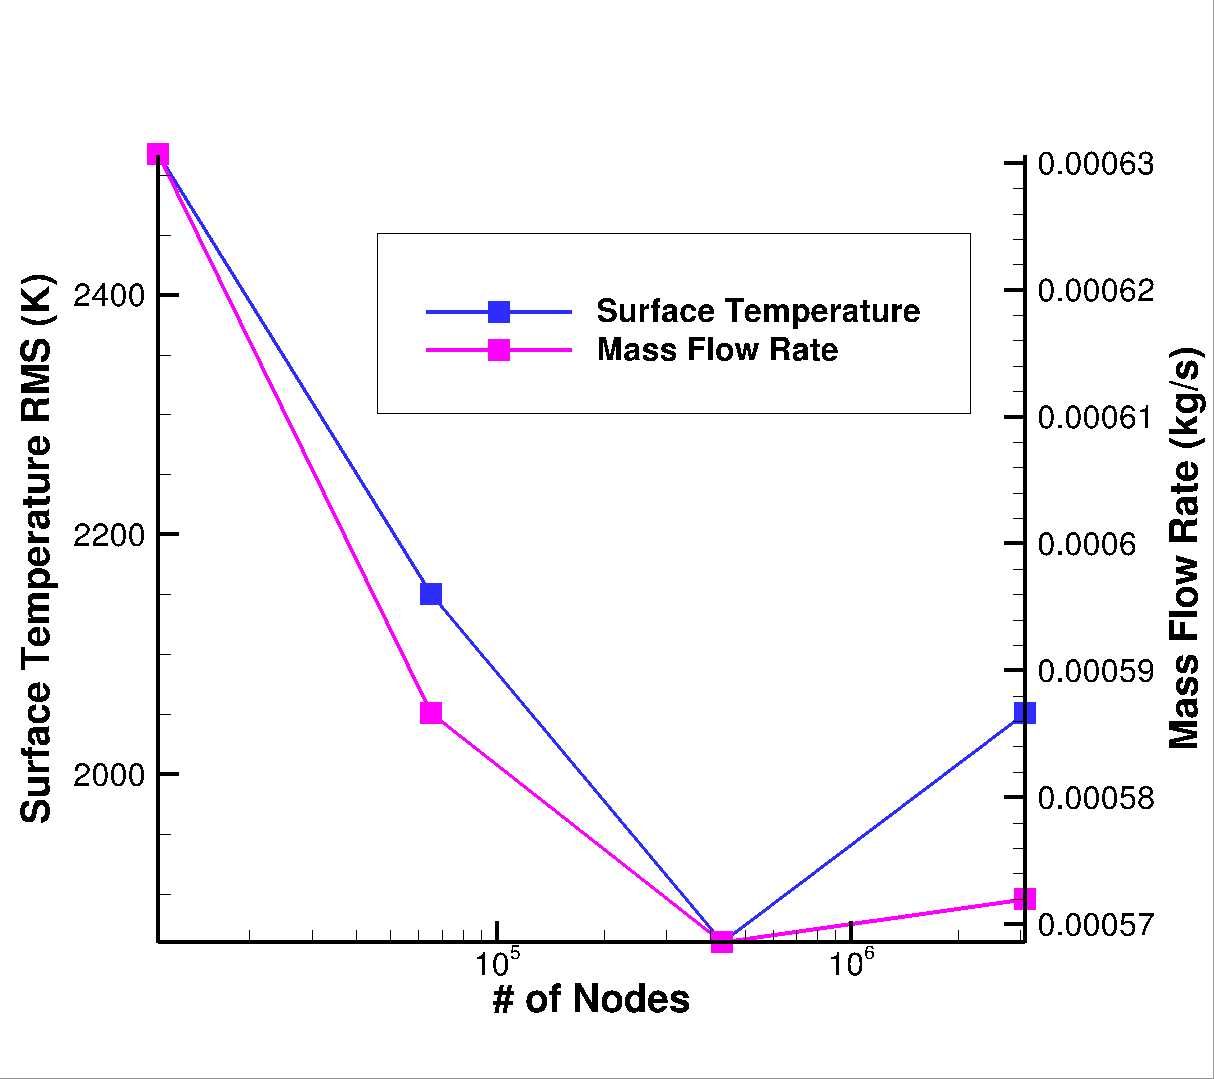
\includegraphics[width=0.75\textwidth]{figures/t-m-conv.png}
  \caption{Surface temperature and plenum mass flow rate.}
\end{figure}
%------------------------------------------------------------------------------%
    \end{column}
  \end{columns}
\end{frame}
\begin{frame}
  \frametitle{Accuracy of the Adjoint Sensitivity Derivatives}
  \begin{itemize}
    \item To verify adjoint, derivatives computed by complex step eliminates
      subtractive cancellation error
%------------------------------------------------------------------------------%
    \[
      \pd{f}{x} = \frac{Im\left[ f(x + ih) \right]}{h} - O(h^2)
    \]
%------------------------------------------------------------------------------%
    \item FUN3D is ``complexified'' by ruby scripting, and sensitivities
      computed by perturbing design variables individually
    \item The complex-value solver is restarted with the real-value flow solver
      solution to avoid recomputing flux limiter
      \begin{itemize}
        \item Ensures that frozen flux limiter values used by adjoint
          solver and complex-value flow solver are identical
      \end{itemize}
  \end{itemize}
\end{frame}
\begin{frame}
  \frametitle{Consistency of Decoupled Flow Solver}
  \begin{itemize}
    \item Decoupled and fully coupled flow solvers produce the same surface
      temperature RMS and almost the same plenum mass flow rate for frozen flow
%------------------------------------------------------------------------------%
\begin{table}
  \centering
  \tiny
  \begin{tabular}{c|c|c|c}
    Quantity & Decoupled & Fully Coupled & Relative Difference \\
    \hline
    $\massflow$ & 0.8450858226893225E-03 & 0.8450858226893034E-03 & 2.26E-14 \\
    $T_{RMS}$   & 0.1508600871984388E+04 & 0.1508600871984388E+04 & 0
  \end{tabular}
  \caption{Difference with frozen chemistry.}
\end{table}
%------------------------------------------------------------------------------%
    \item Comparison degrades for chemically reacting flows, but is consistent
      with the aforementioned relative level of convergence
%------------------------------------------------------------------------------%
\begin{table}
  \tiny
  \centering
  \begin{tabular}{c|c|c|c}
    Quantity & Decoupled & Fully Coupled & Relative Difference \\
    \hline
    $\massflow$ & 0.8448720721551258E-03 & 0.8448720721551088E-03 & 2.01E-14 \\
    $T_{RMS}$   & 0.1545729169703027E+04 & 0.1545720949811712E+04 & 5.32E-06
  \end{tabular}
  \caption{Difference with finite-rate chemistry.}
\end{table}
%------------------------------------------------------------------------------%
  \end{itemize}
\end{frame}
\begin{frame}
  \frametitle{Consistency of Decoupled Adjoint Solver}
  \begin{itemize}
    \item Very good agreement between the sensitivity derivatives computed by
      the decoupled and fully coupled adjoint solvers
%------------------------------------------------------------------------------%
\begin{table}[h]
  \tiny
  \centering
  \begin{tabular}{c|c|c|c}
    Design Variable & Decoupled Sensitivity & Fully Coupled Sensitivity & Rel. Diff\\
    \hline
    $P_{p,o}$ & -0.11081315601976E-06 & -0.11081315649260E-06 & 4E-9  \\
    $T_{p,o}$ &  0.19089941243495E-03 &  0.19089941237390E-03 & 3E-10 \\
    $\fa$     & -0.28035409093945E-01 & -0.28035409045530E-01 & 1E-9
  \end{tabular}
  \caption{Annular jet plenum sensitivity relative difference.}
\end{table}
%------------------------------------------------------------------------------%
    \item All differences less than those in comparison to complex step derivatives
    \item More than sufficient for optimization procedure to converge to the
      same optimal result
  \end{itemize}
\end{frame}

\begin{frame}
  \frametitle{Relative Speedup of Decoupled Flow Solver}
  \begin{itemize}
    \item Reasons for decrease in decoupled flow solver speedup with finite-rate
      chemistry relative to frozen flow:
    \begin{itemize}
      \item Exact linearizations are less effective with the highly non-linear
        chemical source term.
      \item Computing the Jacobian is a dominant cost in the decoupled flow
        solver, and is recomputed more frequently when solution is not
        converging
    \end{itemize}
  \item Future work will focus on improving iterative convergence with
    finite-rate chemistry and optimizing the Jacobian computation 
    \begin{itemize}
      \item Better limiting for hydrogen-air combustion reactions
      \item Force low-level vectorization and function inlining for Jacobian
        routines
    \end{itemize}
  \end{itemize}
\end{frame}

\begin{frame}
  \frametitle{Conclusion - New Performance Opportunities}
  \begin{itemize}
    \item Eliminating the linear solve as the dominant cost enables new avenues
      for performance improvements
      \begin{enumerate}
        \item Fixed $5 \times 5$ problem size is beneficial for compile-time
          optimizations
        \item More ``low hanging fruit'' in optimizing thermo-chemistry and
          Jacobian computations than the linear solver
        \item Adjoint memory co-location can be improved to recover speedup when
          second-order linearizations cannot be stored
      \end{enumerate}
    \item Decoupled flow and adjoint solvers enable the generation of a flow
      solution and sensitivities for a cost function in less time than a fully
      coupled flow solution, for demonstration problem
  \end{itemize}
\end{frame}

\end{document}
